% Options for packages loaded elsewhere
\PassOptionsToPackage{unicode}{hyperref}
\PassOptionsToPackage{hyphens}{url}
%
\documentclass[
]{article}
\usepackage{lmodern}
\usepackage{amssymb,amsmath}
\usepackage{ifxetex,ifluatex}
\ifnum 0\ifxetex 1\fi\ifluatex 1\fi=0 % if pdftex
  \usepackage[T1]{fontenc}
  \usepackage[utf8]{inputenc}
  \usepackage{textcomp} % provide euro and other symbols
\else % if luatex or xetex
  \usepackage{unicode-math}
  \defaultfontfeatures{Scale=MatchLowercase}
  \defaultfontfeatures[\rmfamily]{Ligatures=TeX,Scale=1}
\fi
% Use upquote if available, for straight quotes in verbatim environments
\IfFileExists{upquote.sty}{\usepackage{upquote}}{}
\IfFileExists{microtype.sty}{% use microtype if available
  \usepackage[]{microtype}
  \UseMicrotypeSet[protrusion]{basicmath} % disable protrusion for tt fonts
}{}
\makeatletter
\@ifundefined{KOMAClassName}{% if non-KOMA class
  \IfFileExists{parskip.sty}{%
    \usepackage{parskip}
  }{% else
    \setlength{\parindent}{0pt}
    \setlength{\parskip}{6pt plus 2pt minus 1pt}}
}{% if KOMA class
  \KOMAoptions{parskip=half}}
\makeatother
\usepackage{xcolor}
\IfFileExists{xurl.sty}{\usepackage{xurl}}{} % add URL line breaks if available
\IfFileExists{bookmark.sty}{\usepackage{bookmark}}{\usepackage{hyperref}}
\hypersetup{
  pdftitle={Multistep Model of Parkinson's},
  hidelinks,
  pdfcreator={LaTeX via pandoc}}
\urlstyle{same} % disable monospaced font for URLs
\usepackage[margin=2cm]{geometry}
\usepackage{color}
\usepackage{fancyvrb}
\newcommand{\VerbBar}{|}
\newcommand{\VERB}{\Verb[commandchars=\\\{\}]}
\DefineVerbatimEnvironment{Highlighting}{Verbatim}{commandchars=\\\{\}}
% Add ',fontsize=\small' for more characters per line
\usepackage{framed}
\definecolor{shadecolor}{RGB}{248,248,248}
\newenvironment{Shaded}{\begin{snugshade}}{\end{snugshade}}
\newcommand{\AlertTok}[1]{\textcolor[rgb]{0.94,0.16,0.16}{#1}}
\newcommand{\AnnotationTok}[1]{\textcolor[rgb]{0.56,0.35,0.01}{\textbf{\textit{#1}}}}
\newcommand{\AttributeTok}[1]{\textcolor[rgb]{0.77,0.63,0.00}{#1}}
\newcommand{\BaseNTok}[1]{\textcolor[rgb]{0.00,0.00,0.81}{#1}}
\newcommand{\BuiltInTok}[1]{#1}
\newcommand{\CharTok}[1]{\textcolor[rgb]{0.31,0.60,0.02}{#1}}
\newcommand{\CommentTok}[1]{\textcolor[rgb]{0.56,0.35,0.01}{\textit{#1}}}
\newcommand{\CommentVarTok}[1]{\textcolor[rgb]{0.56,0.35,0.01}{\textbf{\textit{#1}}}}
\newcommand{\ConstantTok}[1]{\textcolor[rgb]{0.00,0.00,0.00}{#1}}
\newcommand{\ControlFlowTok}[1]{\textcolor[rgb]{0.13,0.29,0.53}{\textbf{#1}}}
\newcommand{\DataTypeTok}[1]{\textcolor[rgb]{0.13,0.29,0.53}{#1}}
\newcommand{\DecValTok}[1]{\textcolor[rgb]{0.00,0.00,0.81}{#1}}
\newcommand{\DocumentationTok}[1]{\textcolor[rgb]{0.56,0.35,0.01}{\textbf{\textit{#1}}}}
\newcommand{\ErrorTok}[1]{\textcolor[rgb]{0.64,0.00,0.00}{\textbf{#1}}}
\newcommand{\ExtensionTok}[1]{#1}
\newcommand{\FloatTok}[1]{\textcolor[rgb]{0.00,0.00,0.81}{#1}}
\newcommand{\FunctionTok}[1]{\textcolor[rgb]{0.00,0.00,0.00}{#1}}
\newcommand{\ImportTok}[1]{#1}
\newcommand{\InformationTok}[1]{\textcolor[rgb]{0.56,0.35,0.01}{\textbf{\textit{#1}}}}
\newcommand{\KeywordTok}[1]{\textcolor[rgb]{0.13,0.29,0.53}{\textbf{#1}}}
\newcommand{\NormalTok}[1]{#1}
\newcommand{\OperatorTok}[1]{\textcolor[rgb]{0.81,0.36,0.00}{\textbf{#1}}}
\newcommand{\OtherTok}[1]{\textcolor[rgb]{0.56,0.35,0.01}{#1}}
\newcommand{\PreprocessorTok}[1]{\textcolor[rgb]{0.56,0.35,0.01}{\textit{#1}}}
\newcommand{\RegionMarkerTok}[1]{#1}
\newcommand{\SpecialCharTok}[1]{\textcolor[rgb]{0.00,0.00,0.00}{#1}}
\newcommand{\SpecialStringTok}[1]{\textcolor[rgb]{0.31,0.60,0.02}{#1}}
\newcommand{\StringTok}[1]{\textcolor[rgb]{0.31,0.60,0.02}{#1}}
\newcommand{\VariableTok}[1]{\textcolor[rgb]{0.00,0.00,0.00}{#1}}
\newcommand{\VerbatimStringTok}[1]{\textcolor[rgb]{0.31,0.60,0.02}{#1}}
\newcommand{\WarningTok}[1]{\textcolor[rgb]{0.56,0.35,0.01}{\textbf{\textit{#1}}}}
\usepackage{graphicx,grffile}
\makeatletter
\def\maxwidth{\ifdim\Gin@nat@width>\linewidth\linewidth\else\Gin@nat@width\fi}
\def\maxheight{\ifdim\Gin@nat@height>\textheight\textheight\else\Gin@nat@height\fi}
\makeatother
% Scale images if necessary, so that they will not overflow the page
% margins by default, and it is still possible to overwrite the defaults
% using explicit options in \includegraphics[width, height, ...]{}
\setkeys{Gin}{width=\maxwidth,height=\maxheight,keepaspectratio}
% Set default figure placement to htbp
\makeatletter
\def\fps@figure{htbp}
\makeatother
\setlength{\emergencystretch}{3em} % prevent overfull lines
\providecommand{\tightlist}{%
  \setlength{\itemsep}{0pt}\setlength{\parskip}{0pt}}
\setcounter{secnumdepth}{-\maxdimen} % remove section numbering
\usepackage{hyperref}

\title{Multistep Model of Parkinson's}
\author{}
\date{\vspace{-2.5em}}

\begin{document}
\maketitle

\hypertarget{r-setup}{%
\subsection{R Setup}\label{r-setup}}

\hypertarget{data-import}{%
\subsection{Data import}\label{data-import}}

\begin{Shaded}
\begin{Highlighting}[]
\NormalTok{ages_}\DecValTok{100}\NormalTok{ <-}\StringTok{ }\KeywordTok{c}\NormalTok{(}\StringTok{"30"}\NormalTok{,}\StringTok{"35"}\NormalTok{,}\StringTok{"40"}\NormalTok{,}\StringTok{"45"}\NormalTok{,}\StringTok{"50"}\NormalTok{,}\StringTok{"55"}\NormalTok{,}
              \StringTok{"60"}\NormalTok{,}\StringTok{"65"}\NormalTok{,}\StringTok{"70"}\NormalTok{,}\StringTok{"75"}\NormalTok{,}\StringTok{"80"}\NormalTok{,}
              \StringTok{"85"}\NormalTok{,}\StringTok{"90"}\NormalTok{,}\StringTok{"95"}\NormalTok{,}\StringTok{"100+"}\NormalTok{)}

\NormalTok{sim_df_ms_full <-}\StringTok{ }\KeywordTok{read.csv}\NormalTok{(}\StringTok{"data/incidence_by_age_multistep_full.csv"}\NormalTok{) }\OperatorTok
\StringTok{  }\KeywordTok{mutate}\NormalTok{(}\DataTypeTok{agecut5 =} \KeywordTok{fct_relevel}\NormalTok{(agecut5,ages_}\DecValTok{100}\NormalTok{)) }\OperatorTok
\StringTok{  }\KeywordTok{mutate}\NormalTok{(}\DataTypeTok{agecut5_scaled =}\NormalTok{ agecut5_log}\OperatorTok{-}\KeywordTok{min}\NormalTok{(agecut5_log)) }\OperatorTok
\StringTok{  }\KeywordTok{mutate}\NormalTok{(}\DataTypeTok{restriction =} \KeywordTok{if_else}\NormalTok{(agecut5_numeric}\OperatorTok{<=}\DecValTok{80}\NormalTok{,}\StringTok{"modelled"}\NormalTok{,}\StringTok{"unmodelled"}\NormalTok{))}

\NormalTok{sim_df_ms_sex_full <-}\StringTok{ }\KeywordTok{read.csv}\NormalTok{(}\StringTok{"data/incidence_by_age_multistep_sex_full.csv"}\NormalTok{) }\OperatorTok
\StringTok{  }\KeywordTok{mutate}\NormalTok{(}\DataTypeTok{agecut5 =} \KeywordTok{fct_relevel}\NormalTok{(agecut5,ages_}\DecValTok{100}\NormalTok{)) }\OperatorTok
\StringTok{  }\KeywordTok{filter}\NormalTok{(agecut5_numeric }\OperatorTok{>=}\StringTok{ }\DecValTok{30}\NormalTok{) }\OperatorTok
\StringTok{  }\KeywordTok{mutate}\NormalTok{(}\DataTypeTok{agecut5_scaled =}\NormalTok{ agecut5_log}\OperatorTok{-}\KeywordTok{min}\NormalTok{(agecut5_log)) }\OperatorTok
\StringTok{  }\KeywordTok{mutate}\NormalTok{(}\DataTypeTok{restriction =} \KeywordTok{if_else}\NormalTok{(agecut5_numeric}\OperatorTok{<=}\DecValTok{80}\NormalTok{,}\StringTok{"modelled"}\NormalTok{,}\StringTok{"unmodelled"}\NormalTok{)) }\OperatorTok
\StringTok{  }\KeywordTok{mutate}\NormalTok{(}\DataTypeTok{sex_restriction =} \KeywordTok{factor}\NormalTok{(sex)}\OperatorTok{:}\KeywordTok{factor}\NormalTok{(restriction)) }\OperatorTok
\StringTok{  }\KeywordTok{mutate}\NormalTok{(}\DataTypeTok{sex =} \KeywordTok{factor}\NormalTok{(sex,}\DataTypeTok{levels=}\KeywordTok{c}\NormalTok{(}\StringTok{"Male"}\NormalTok{,}\StringTok{"Female"}\NormalTok{))) }\OperatorTok
\StringTok{  }\KeywordTok{mutate}\NormalTok{(}\DataTypeTok{sex_restriction =} \KeywordTok{factor}\NormalTok{(sex_restriction,}
                \DataTypeTok{levels=}\KeywordTok{c}\NormalTok{(}\StringTok{"Male:modelled"}\NormalTok{,}\StringTok{"Female:modelled"}\NormalTok{,}
                 \StringTok{"Male:unmodelled"}\NormalTok{,}\StringTok{"Female:unmodelled"}\NormalTok{)))}

\NormalTok{sim_df_ms_model <-}\StringTok{ }\NormalTok{sim_df_ms_full }\OperatorTok
\StringTok{  }\KeywordTok{filter}\NormalTok{(agecut5_numeric }\OperatorTok{<=}\StringTok{ }\DecValTok{80}\NormalTok{) }
  
\NormalTok{sim_df_ms_sex_model <-}\StringTok{ }\NormalTok{sim_df_ms_sex_full }\OperatorTok
\StringTok{  }\KeywordTok{filter}\NormalTok{(agecut5_numeric }\OperatorTok{<=}\StringTok{ }\DecValTok{80}\NormalTok{)}
\end{Highlighting}
\end{Shaded}

\hypertarget{common-constantscode}{%
\subsection{Common constants/code}\label{common-constantscode}}

\begin{Shaded}
\begin{Highlighting}[]
\CommentTok{# Colours for modeled/unmodeled data points}
\NormalTok{colours_modelled <-}\StringTok{ }\KeywordTok{c}\NormalTok{(}\StringTok{"#000000"}\NormalTok{, }\StringTok{"#AAAAAA"}\NormalTok{)}

\CommentTok{# Colours for male/female}
\NormalTok{colours_mf <-}\StringTok{ }\KeywordTok{c}\NormalTok{(}\StringTok{"#009E73"}\NormalTok{, }\StringTok{"#D55E00"}\NormalTok{)}

\CommentTok{# Colours for male/female modeled/unmodeled}
\NormalTok{colours_mf_modelled <-}\StringTok{ }\KeywordTok{c}\NormalTok{(}\StringTok{"#009E73"}\NormalTok{, }\StringTok{"#D55E00"}\NormalTok{, }\StringTok{"#AAAAAA"}\NormalTok{, }\StringTok{"#AAAAAA"}\NormalTok{)}
\end{Highlighting}
\end{Shaded}

\hypertarget{model-linear}{%
\subsection{Model: Linear}\label{model-linear}}

\begin{Shaded}
\begin{Highlighting}[]
\NormalTok{mod_ms_linear <-}\StringTok{ }\KeywordTok{stan_model}\NormalTok{(}\StringTok{'stan/multistep_linear.stan'}\NormalTok{)}

\NormalTok{pars_linear <-}\StringTok{ }\KeywordTok{c}\NormalTok{(}\StringTok{'m'}\NormalTok{,}\StringTok{'c'}\NormalTok{,}\StringTok{'sigma_sq'}\NormalTok{)}

\NormalTok{data_list_linear <-}\StringTok{ }\KeywordTok{list}\NormalTok{(}\DataTypeTok{m_prior_mean =} \DecValTok{6}\NormalTok{,}
                  \DataTypeTok{m_prior_sd =} \DecValTok{1}\NormalTok{,}
                  \DataTypeTok{N=}\KeywordTok{nrow}\NormalTok{(sim_df_ms_model),}
                  \DataTypeTok{x =}\NormalTok{ sim_df_ms_model}\OperatorTok{$}\NormalTok{agecut5_scaled, }
                  \DataTypeTok{y_min =}\NormalTok{ sim_df_ms_model}\OperatorTok{$}\NormalTok{lower_log,}
                  \DataTypeTok{y_max =}\NormalTok{ sim_df_ms_model}\OperatorTok{$}\NormalTok{upper_log)}

\NormalTok{fit_linear <-}\StringTok{ }\KeywordTok{sampling}\NormalTok{(mod_ms_linear, }\DataTypeTok{data =}\NormalTok{ data_list_linear, }\DataTypeTok{seed =}\NormalTok{ SEED,}
                   \DataTypeTok{pars =}\NormalTok{ pars_linear, }\DataTypeTok{chains =} \DecValTok{4}\NormalTok{, }\DataTypeTok{iter =} \DecValTok{2000}\NormalTok{,}
                   \DataTypeTok{control =} \KeywordTok{list}\NormalTok{(}\DataTypeTok{max_treedepth =} \DecValTok{15}\NormalTok{,}\DataTypeTok{adapt_delta=}\FloatTok{0.99}\NormalTok{),}
                   \DataTypeTok{verbose=}\OtherTok{TRUE}\NormalTok{)}
\end{Highlighting}
\end{Shaded}

\begin{verbatim}
## 
## CHECKING DATA AND PREPROCESSING FOR MODEL 'multistep_linear' NOW.
## 
## COMPILING MODEL 'multistep_linear' NOW.
## 
## STARTING SAMPLER FOR MODEL 'multistep_linear' NOW.
\end{verbatim}

\begin{Shaded}
\begin{Highlighting}[]
\KeywordTok{print}\NormalTok{(fit_linear)}
\end{Highlighting}
\end{Shaded}

\begin{verbatim}
## Inference for Stan model: multistep_linear.
## 4 chains, each with iter=2000; warmup=1000; thin=1; 
## post-warmup draws per chain=1000, total post-warmup draws=4000.
## 
##            mean se_mean   sd   2.5%    25%   50%   75% 97.5% n_eff Rhat
## m          6.49    0.00 0.12   6.21   6.42  6.51  6.57  6.69   868 1.00
## c         -0.60    0.00 0.09  -0.74  -0.66 -0.61 -0.55 -0.39   916 1.00
## sigma_sq   0.01    0.00 0.01   0.00   0.00  0.01  0.01  0.02   813 1.01
## lp__     -10.22    0.05 1.35 -13.67 -10.85 -9.91 -9.20 -8.64   750 1.00
## 
## Samples were drawn using NUTS(diag_e) at Thu Dec 17 10:15:40 2020.
## For each parameter, n_eff is a crude measure of effective sample size,
## and Rhat is the potential scale reduction factor on split chains (at 
## convergence, Rhat=1).
\end{verbatim}

\begin{Shaded}
\begin{Highlighting}[]
\NormalTok{H_LINEAR =}\StringTok{ }\KeywordTok{bridge_sampler}\NormalTok{(fit_linear)}
\end{Highlighting}
\end{Shaded}

\begin{verbatim}
## Iteration: 1
## Iteration: 2
## Iteration: 3
## Iteration: 4
## Iteration: 5
## Iteration: 6
## Iteration: 7
## Iteration: 8
## Iteration: 9
## Iteration: 10
\end{verbatim}

\hypertarget{model-broken-stick}{%
\subsection{Model: Broken-stick}\label{model-broken-stick}}

\begin{Shaded}
\begin{Highlighting}[]
\NormalTok{mod_ms_bs <-}\StringTok{ }\KeywordTok{stan_model}\NormalTok{(}\StringTok{'stan/multistep_brokenstick.stan'}\NormalTok{)}

\NormalTok{pars_bs <-}\StringTok{ }\KeywordTok{c}\NormalTok{(}\StringTok{'m_early'}\NormalTok{,}\StringTok{'m_late'}\NormalTok{,}\StringTok{'bp'}\NormalTok{,}\StringTok{'c'}\NormalTok{,}\StringTok{'sigma_sq'}\NormalTok{)}

\CommentTok{# wider priors for estimation}
\NormalTok{data_list_bs <-}\StringTok{ }\KeywordTok{list}\NormalTok{(}\DataTypeTok{m_early_prior_mean =} \DecValTok{5}\NormalTok{,}
                     \DataTypeTok{m_early_prior_sd =} \DecValTok{1}\NormalTok{,}
                     \DataTypeTok{m_late_prior_mean =} \DecValTok{7}\NormalTok{,}
                     \DataTypeTok{m_late_prior_sd =} \DecValTok{1}\NormalTok{,}
                     \DataTypeTok{bp_prior_mean =} \FloatTok{0.5}\NormalTok{,}
                     \DataTypeTok{bp_prior_sd =} \FloatTok{0.3}\NormalTok{,}
                     \DataTypeTok{N=}\KeywordTok{nrow}\NormalTok{(sim_df_ms_model),}
                     \DataTypeTok{x =}\NormalTok{ sim_df_ms_model}\OperatorTok{$}\NormalTok{agecut5_scaled, }
                     \DataTypeTok{y_min =}\NormalTok{ sim_df_ms_model}\OperatorTok{$}\NormalTok{lower_log,}
                     \DataTypeTok{y_max =}\NormalTok{ sim_df_ms_model}\OperatorTok{$}\NormalTok{upper_log)}

\NormalTok{fit_bs <-}\StringTok{ }\KeywordTok{sampling}\NormalTok{(mod_ms_bs, }\DataTypeTok{data =}\NormalTok{ data_list_bs, }\DataTypeTok{seed =}\NormalTok{ SEED,}
                  \DataTypeTok{pars =}\NormalTok{ pars_bs, }\DataTypeTok{chains =} \DecValTok{4}\NormalTok{, }\DataTypeTok{iter =} \DecValTok{2000}\NormalTok{,}
                  \DataTypeTok{control =} \KeywordTok{list}\NormalTok{(}\DataTypeTok{max_treedepth =} \DecValTok{15}\NormalTok{,}\DataTypeTok{adapt_delta=}\FloatTok{0.99}\NormalTok{),}
                  \DataTypeTok{verbose=}\OtherTok{TRUE}\NormalTok{)}
\end{Highlighting}
\end{Shaded}

\begin{verbatim}
## 
## CHECKING DATA AND PREPROCESSING FOR MODEL 'multistep_brokenstick' NOW.
## 
## COMPILING MODEL 'multistep_brokenstick' NOW.
## 
## STARTING SAMPLER FOR MODEL 'multistep_brokenstick' NOW.
\end{verbatim}

\begin{Shaded}
\begin{Highlighting}[]
\KeywordTok{print}\NormalTok{(fit_bs)}
\end{Highlighting}
\end{Shaded}

\begin{verbatim}
## Inference for Stan model: multistep_brokenstick.
## 4 chains, each with iter=2000; warmup=1000; thin=1; 
## post-warmup draws per chain=1000, total post-warmup draws=4000.
## 
##            mean se_mean   sd   2.5%    25%    50%    75% 97.5% n_eff Rhat
## m_early    5.21    0.02 0.70   3.78   4.74   5.23   5.72  6.44  1296 1.00
## m_late     6.75    0.01 0.21   6.37   6.61   6.73   6.87  7.21  1327 1.00
## bp         0.41    0.00 0.11   0.22   0.34   0.41   0.48  0.65  1282 1.00
## c         -0.20    0.01 0.22  -0.62  -0.37  -0.20  -0.04  0.22  1165 1.00
## sigma_sq   0.01    0.00 0.01   0.00   0.00   0.01   0.01  0.02  1153 1.01
## lp__     -11.80    0.06 1.86 -16.39 -12.79 -11.37 -10.42 -9.44   865 1.00
## 
## Samples were drawn using NUTS(diag_e) at Thu Dec 17 10:15:42 2020.
## For each parameter, n_eff is a crude measure of effective sample size,
## and Rhat is the potential scale reduction factor on split chains (at 
## convergence, Rhat=1).
\end{verbatim}

\begin{Shaded}
\begin{Highlighting}[]
\CommentTok{## Run in console}
\CommentTok{#pdf("plots/bs_pairs_diagnosis.pdf")}
\CommentTok{#pairs(fit_bs)}
\CommentTok{#dev.off()}

\NormalTok{H_BS =}\StringTok{ }\KeywordTok{bridge_sampler}\NormalTok{(fit_bs)}
\end{Highlighting}
\end{Shaded}

\begin{verbatim}
## Warning: 14 of the 2000 log_prob() evaluations on the proposal draws produced
## -Inf/Inf.
\end{verbatim}

\begin{verbatim}
## Iteration: 1
## Iteration: 2
## Iteration: 3
## Iteration: 4
## Iteration: 5
## Iteration: 6
## Iteration: 7
## Iteration: 8
## Iteration: 9
## Iteration: 10
## Iteration: 11
\end{verbatim}

\begin{Shaded}
\begin{Highlighting}[]
\NormalTok{bf_bs =}\StringTok{ }\KeywordTok{bf}\NormalTok{(H_BS,H_LINEAR)}
\end{Highlighting}
\end{Shaded}

\hypertarget{model-sex-broken-stick}{%
\subsection{Model: Sex Broken-stick}\label{model-sex-broken-stick}}

\begin{Shaded}
\begin{Highlighting}[]
\CommentTok{# Common slope and intercept by sex}
\NormalTok{mod_ms_bs_sex_common <-}\StringTok{ }\KeywordTok{stan_model}\NormalTok{(}\StringTok{'stan/multistep_brokenstick.stan'}\NormalTok{)}
\NormalTok{pars_bs_sex_common <-}\StringTok{ }\KeywordTok{c}\NormalTok{(}\StringTok{'m_early'}\NormalTok{,}\StringTok{'m_late'}\NormalTok{,}\StringTok{'bp'}\NormalTok{,}\StringTok{'c'}\NormalTok{,}\StringTok{'sigma_sq'}\NormalTok{)}

\CommentTok{# Allow intercept vary by sex}
\NormalTok{mod_ms_bs_sex_vc <-}\StringTok{ }\KeywordTok{stan_model}\NormalTok{(}\StringTok{'stan/multistep_brokenstick_sex_intercept.stan'}\NormalTok{)}
\NormalTok{pars_bs_sex_vc <-}\StringTok{ }\KeywordTok{c}\NormalTok{(}\StringTok{'m_early'}\NormalTok{,}\StringTok{'m_late'}\NormalTok{,}\StringTok{'bp'}\NormalTok{,}\StringTok{'c'}\NormalTok{,}\StringTok{'c_sex'}\NormalTok{,}\StringTok{'sigma_sq'}\NormalTok{)}

\CommentTok{# Allow slope and intercept to vary by sex}
\NormalTok{mod_ms_bs_sex_vmc <-}\StringTok{ }\KeywordTok{stan_model}\NormalTok{(}\StringTok{'stan/multistep_brokenstick_sex.stan'}\NormalTok{)}
\NormalTok{pars_bs_sex_vmc <-}\StringTok{ }\KeywordTok{c}\NormalTok{(}\StringTok{'m_early'}\NormalTok{,}\StringTok{'m_late'}\NormalTok{,}\StringTok{'bp'}\NormalTok{,}\StringTok{'c'}\NormalTok{,}\StringTok{'c_sex'}\NormalTok{,}\StringTok{'m_sex'}\NormalTok{,}\StringTok{'sigma_sq'}\NormalTok{,}
                    \StringTok{'c_female'}\NormalTok{,}\StringTok{'m_early_female'}\NormalTok{,}\StringTok{'m_late_female'}\NormalTok{)}

\CommentTok{# data and priors - varying intercept/slope}
\NormalTok{data_list_bs_sex <-}\StringTok{ }\KeywordTok{list}\NormalTok{(}\DataTypeTok{m_early_prior_mean =} \DecValTok{5}\NormalTok{,}
                     \DataTypeTok{m_early_prior_sd =} \DecValTok{1}\NormalTok{,}
                     \DataTypeTok{m_late_prior_mean =} \DecValTok{7}\NormalTok{,}
                     \DataTypeTok{m_late_prior_sd =} \DecValTok{1}\NormalTok{,}
                     \DataTypeTok{bp_prior_mean =} \FloatTok{0.5}\NormalTok{,}
                     \DataTypeTok{bp_prior_sd =} \FloatTok{0.3}\NormalTok{,}
                     \DataTypeTok{N=}\KeywordTok{nrow}\NormalTok{(sim_df_ms_sex_model),}
                     \DataTypeTok{x =}\NormalTok{ sim_df_ms_sex_model}\OperatorTok{$}\NormalTok{agecut5_scaled,}
                     \DataTypeTok{sex =} \KeywordTok{abs}\NormalTok{(}\KeywordTok{as.numeric}\NormalTok{(}\KeywordTok{factor}\NormalTok{(sim_df_ms_sex_model}\OperatorTok{$}\NormalTok{sex))}\OperatorTok{-}\DecValTok{2}\NormalTok{),}
                     \DataTypeTok{y_min =}\NormalTok{ sim_df_ms_sex_model}\OperatorTok{$}\NormalTok{lower_log,}
                     \DataTypeTok{y_max =}\NormalTok{ sim_df_ms_sex_model}\OperatorTok{$}\NormalTok{upper_log)}

\CommentTok{# Common slope and intercept to vary by sex}
\NormalTok{fit_bs_sex_common <-}\StringTok{ }\KeywordTok{sampling}\NormalTok{(mod_ms_bs_sex_common, }\DataTypeTok{data =}\NormalTok{ data_list_bs_sex, }
                  \DataTypeTok{seed =}\NormalTok{ SEED,}
                  \DataTypeTok{pars =}\NormalTok{ pars_bs_sex_common, }\DataTypeTok{chains =} \DecValTok{4}\NormalTok{, }\DataTypeTok{iter =} \DecValTok{2000}\NormalTok{,}
                  \DataTypeTok{control =} \KeywordTok{list}\NormalTok{(}\DataTypeTok{max_treedepth =} \DecValTok{20}\NormalTok{,}\DataTypeTok{adapt_delta=}\FloatTok{0.99}\NormalTok{),}
                  \DataTypeTok{verbose=}\OtherTok{TRUE}\NormalTok{)}
\end{Highlighting}
\end{Shaded}

\begin{verbatim}
## 
## CHECKING DATA AND PREPROCESSING FOR MODEL 'multistep_brokenstick' NOW.
## 
## COMPILING MODEL 'multistep_brokenstick' NOW.
## 
## STARTING SAMPLER FOR MODEL 'multistep_brokenstick' NOW.
\end{verbatim}

\begin{Shaded}
\begin{Highlighting}[]
\KeywordTok{print}\NormalTok{(fit_bs_sex_common)}
\end{Highlighting}
\end{Shaded}

\begin{verbatim}
## Inference for Stan model: multistep_brokenstick.
## 4 chains, each with iter=2000; warmup=1000; thin=1; 
## post-warmup draws per chain=1000, total post-warmup draws=4000.
## 
##            mean se_mean   sd   2.5%    25%    50%    75%  97.5% n_eff Rhat
## m_early    5.25    0.02 0.71   3.74   4.78   5.30   5.77   6.48  1542    1
## m_late     6.86    0.01 0.45   6.09   6.55   6.82   7.13   7.84  1888    1
## bp         0.46    0.00 0.14   0.22   0.35   0.45   0.55   0.75  1724    1
## c         -0.21    0.01 0.22  -0.64  -0.36  -0.21  -0.06   0.22  1776    1
## sigma_sq   0.09    0.00 0.03   0.04   0.06   0.08   0.10   0.17  2037    1
## lp__     -38.42    0.05 1.83 -42.79 -39.35 -38.07 -37.11 -35.93  1136    1
## 
## Samples were drawn using NUTS(diag_e) at Thu Dec 17 10:15:44 2020.
## For each parameter, n_eff is a crude measure of effective sample size,
## and Rhat is the potential scale reduction factor on split chains (at 
## convergence, Rhat=1).
\end{verbatim}

\begin{Shaded}
\begin{Highlighting}[]
\CommentTok{# Allow intercept to vary by sex}
\NormalTok{fit_bs_sex_vc <-}\StringTok{ }\KeywordTok{sampling}\NormalTok{(mod_ms_bs_sex_vc, }\DataTypeTok{data =}\NormalTok{ data_list_bs_sex, }
                  \DataTypeTok{seed =}\NormalTok{ SEED,}
                  \DataTypeTok{pars =}\NormalTok{ pars_bs_sex_vc, }\DataTypeTok{chains =} \DecValTok{4}\NormalTok{, }\DataTypeTok{iter =} \DecValTok{2000}\NormalTok{,}
                  \DataTypeTok{control =} \KeywordTok{list}\NormalTok{(}\DataTypeTok{max_treedepth =} \DecValTok{20}\NormalTok{,}\DataTypeTok{adapt_delta=}\FloatTok{0.99}\NormalTok{),}
                  \DataTypeTok{verbose=}\OtherTok{TRUE}\NormalTok{)}
\end{Highlighting}
\end{Shaded}

\begin{verbatim}
## 
## CHECKING DATA AND PREPROCESSING FOR MODEL 'multistep_brokenstick_sex_intercept' NOW.
## 
## COMPILING MODEL 'multistep_brokenstick_sex_intercept' NOW.
## 
## STARTING SAMPLER FOR MODEL 'multistep_brokenstick_sex_intercept' NOW.
\end{verbatim}

\begin{Shaded}
\begin{Highlighting}[]
\KeywordTok{print}\NormalTok{(fit_bs_sex_vc)}
\end{Highlighting}
\end{Shaded}

\begin{verbatim}
## Inference for Stan model: multistep_brokenstick_sex_intercept.
## 4 chains, each with iter=2000; warmup=1000; thin=1; 
## post-warmup draws per chain=1000, total post-warmup draws=4000.
## 
##            mean se_mean   sd   2.5%    25%    50%    75%  97.5% n_eff Rhat
## m_early    5.18    0.02 0.66   3.76   4.73   5.21   5.69   6.32  1351    1
## m_late     6.75    0.00 0.15   6.49   6.65   6.74   6.84   7.07  1951    1
## bp         0.40    0.00 0.09   0.22   0.33   0.40   0.46   0.59  1654    1
## c         -0.49    0.01 0.21  -0.87  -0.65  -0.49  -0.33  -0.11  1348    1
## c_sex      0.53    0.00 0.04   0.45   0.50   0.53   0.56   0.61  2265    1
## sigma_sq   0.00    0.00 0.00   0.00   0.00   0.00   0.01   0.01  1911    1
## lp__     -14.90    0.05 1.88 -19.52 -15.95 -14.54 -13.47 -12.34  1210    1
## 
## Samples were drawn using NUTS(diag_e) at Thu Dec 17 10:15:47 2020.
## For each parameter, n_eff is a crude measure of effective sample size,
## and Rhat is the potential scale reduction factor on split chains (at 
## convergence, Rhat=1).
\end{verbatim}

\begin{Shaded}
\begin{Highlighting}[]
\CommentTok{# Allow slope and intercept to vary by sex}
\NormalTok{fit_bs_sex_vmc <-}\StringTok{ }\KeywordTok{sampling}\NormalTok{(mod_ms_bs_sex_vmc, }\DataTypeTok{data =}\NormalTok{ data_list_bs_sex, }
                  \DataTypeTok{seed =}\NormalTok{ SEED,}
                  \DataTypeTok{pars =}\NormalTok{ pars_bs_sex_vmc, }\DataTypeTok{chains =} \DecValTok{4}\NormalTok{, }\DataTypeTok{iter =} \DecValTok{2000}\NormalTok{,}
                  \DataTypeTok{control =} \KeywordTok{list}\NormalTok{(}\DataTypeTok{max_treedepth =} \DecValTok{20}\NormalTok{,}\DataTypeTok{adapt_delta=}\FloatTok{0.99}\NormalTok{),}
                  \DataTypeTok{verbose=}\OtherTok{TRUE}\NormalTok{)}
\end{Highlighting}
\end{Shaded}

\begin{verbatim}
## 
## CHECKING DATA AND PREPROCESSING FOR MODEL 'multistep_brokenstick_sex' NOW.
## 
## COMPILING MODEL 'multistep_brokenstick_sex' NOW.
## 
## STARTING SAMPLER FOR MODEL 'multistep_brokenstick_sex' NOW.
\end{verbatim}

\begin{Shaded}
\begin{Highlighting}[]
\KeywordTok{print}\NormalTok{(fit_bs_sex_vmc)}
\end{Highlighting}
\end{Shaded}

\begin{verbatim}
## Inference for Stan model: multistep_brokenstick_sex.
## 4 chains, each with iter=2000; warmup=1000; thin=1; 
## post-warmup draws per chain=1000, total post-warmup draws=4000.
## 
##                  mean se_mean   sd   2.5%    25%    50%    75%  97.5% n_eff
## m_early          5.13    0.02 0.65   3.78   4.70   5.15   5.59   6.28  1506
## m_late           6.74    0.00 0.19   6.38   6.61   6.73   6.86   7.12  1704
## bp               0.40    0.00 0.09   0.23   0.34   0.40   0.46   0.59  1734
## c               -0.46    0.01 0.23  -0.88  -0.63  -0.46  -0.29  -0.03  1366
## c_sex            0.50    0.00 0.17   0.16   0.38   0.50   0.61   0.86  1309
## m_sex            0.04    0.01 0.23  -0.43  -0.11   0.04   0.18   0.48  1301
## sigma_sq         0.01    0.00 0.00   0.00   0.00   0.00   0.01   0.01  1813
## c_female         0.04    0.00 0.21  -0.35  -0.11   0.04   0.20   0.41  1777
## m_early_female   5.17    0.02 0.65   3.81   4.73   5.20   5.64   6.32  1655
## m_late_female    6.77    0.00 0.18   6.44   6.65   6.77   6.88   7.15  2265
## lp__           -15.26    0.06 2.07 -20.23 -16.42 -14.87 -13.72 -12.40  1148
##                Rhat
## m_early           1
## m_late            1
## bp                1
## c                 1
## c_sex             1
## m_sex             1
## sigma_sq          1
## c_female          1
## m_early_female    1
## m_late_female     1
## lp__              1
## 
## Samples were drawn using NUTS(diag_e) at Thu Dec 17 10:15:50 2020.
## For each parameter, n_eff is a crude measure of effective sample size,
## and Rhat is the potential scale reduction factor on split chains (at 
## convergence, Rhat=1).
\end{verbatim}

\begin{Shaded}
\begin{Highlighting}[]
\CommentTok{## DIAGNOSITICS}
\CommentTok{## Run in console}
\CommentTok{#pdf("plots/sex_pairs_diagnosis.pdf")}
\CommentTok{#pairs(fit_bs_sex_vmc)}
\CommentTok{#dev.off()}

\NormalTok{H_BS_SEX_COMMON =}\StringTok{ }\KeywordTok{bridge_sampler}\NormalTok{(fit_bs_sex_common)}
\end{Highlighting}
\end{Shaded}

\begin{verbatim}
## Iteration: 1
## Iteration: 2
## Iteration: 3
## Iteration: 4
## Iteration: 5
## Iteration: 6
## Iteration: 7
## Iteration: 8
\end{verbatim}

\begin{Shaded}
\begin{Highlighting}[]
\NormalTok{H_BS_SEX_VC =}\StringTok{ }\KeywordTok{bridge_sampler}\NormalTok{(fit_bs_sex_vc)}
\end{Highlighting}
\end{Shaded}

\begin{verbatim}
## Warning: 5 of the 2000 log_prob() evaluations on the proposal draws produced
## -Inf/Inf.
\end{verbatim}

\begin{verbatim}
## Iteration: 1
## Iteration: 2
## Iteration: 3
## Iteration: 4
## Iteration: 5
## Iteration: 6
## Iteration: 7
## Iteration: 8
## Iteration: 9
## Iteration: 10
\end{verbatim}

\begin{Shaded}
\begin{Highlighting}[]
\NormalTok{H_BS_SEX_VMC =}\StringTok{ }\KeywordTok{bridge_sampler}\NormalTok{(fit_bs_sex_vmc)}
\end{Highlighting}
\end{Shaded}

\begin{verbatim}
## Warning: 2 of the 2000 log_prob() evaluations on the proposal draws produced
## -Inf/Inf.
\end{verbatim}

\begin{verbatim}
## Iteration: 1
## Iteration: 2
## Iteration: 3
## Iteration: 4
## Iteration: 5
## Iteration: 6
## Iteration: 7
## Iteration: 8
## Iteration: 9
## Iteration: 10
\end{verbatim}

\begin{Shaded}
\begin{Highlighting}[]
\KeywordTok{bf}\NormalTok{(H_BS_SEX_VC,H_BS_SEX_COMMON)}
\end{Highlighting}
\end{Shaded}

\begin{verbatim}
## Estimated Bayes factor in favor of H_BS_SEX_VC over H_BS_SEX_COMMON: 209889691.01172
\end{verbatim}

\begin{Shaded}
\begin{Highlighting}[]
\KeywordTok{bf}\NormalTok{(H_BS_SEX_VMC,H_BS_SEX_VC)}
\end{Highlighting}
\end{Shaded}

\begin{verbatim}
## Estimated Bayes factor in favor of H_BS_SEX_VMC over H_BS_SEX_VC: 0.03939
\end{verbatim}

\hypertarget{model-armitage-doll}{%
\subsection{Model: Armitage-Doll}\label{model-armitage-doll}}

\begin{verbatim}
## 
## Formula: middle ~ (alpha * agecut5_numeric)^(k - 1) * 1e+05
## 
## Parameters:
##        Estimate Std. Error t value Pr(>|t|)    
## alpha 0.0047029  0.0002309   20.37 7.72e-09 ***
## k     6.9154990  0.2815963   24.56 1.47e-09 ***
## ---
## Signif. codes:  0 '***' 0.001 '**' 0.01 '*' 0.05 '.' 0.1 ' ' 1
## 
## Residual standard error: 8.861 on 9 degrees of freedom
## 
## Number of iterations to convergence: 6 
## Achieved convergence tolerance: 8.947e-06
\end{verbatim}

\begin{verbatim}
## 
## CHECKING DATA AND PREPROCESSING FOR MODEL 'multistep_ad' NOW.
## 
## COMPILING MODEL 'multistep_ad' NOW.
## 
## STARTING SAMPLER FOR MODEL 'multistep_ad' NOW.
\end{verbatim}

\begin{verbatim}
## Inference for Stan model: multistep_ad.
## 4 chains, each with iter=2000; warmup=1000; thin=1; 
## post-warmup draws per chain=1000, total post-warmup draws=4000.
## 
##            mean se_mean   sd   2.5%    25%    50%    75%  97.5% n_eff Rhat
## alpha      4.71    0.00 0.14   4.45   4.62   4.71   4.80   4.99   891 1.00
## k          6.93    0.01 0.17   6.62   6.82   6.93   7.03   7.27   884 1.00
## sigma_sq  28.72    0.17 5.37  19.61  24.97  28.19  32.00  40.51   951 1.00
## lp__     -33.54    0.05 1.29 -37.07 -34.06 -33.18 -32.61 -32.12   760 1.01
## 
## Samples were drawn using NUTS(diag_e) at Thu Dec 17 10:15:53 2020.
## For each parameter, n_eff is a crude measure of effective sample size,
## and Rhat is the potential scale reduction factor on split chains (at 
## convergence, Rhat=1).
\end{verbatim}

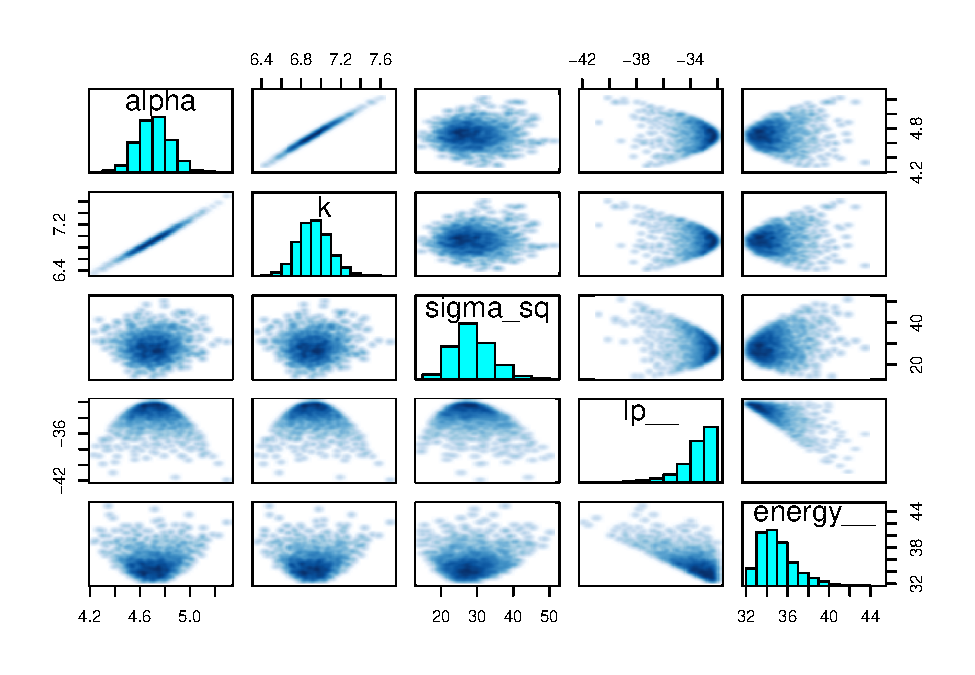
\includegraphics{multistep-model-comparison_files/figure-latex/model_ad-1.pdf}

\begin{verbatim}
## Iteration: 1
## Iteration: 2
## Iteration: 3
## Iteration: 4
## Iteration: 5
## Iteration: 6
\end{verbatim}

\hypertarget{model-armitage-doll-sex}{%
\subsection{Model: Armitage-Doll Sex}\label{model-armitage-doll-sex}}

\begin{verbatim}
## 
## CHECKING DATA AND PREPROCESSING FOR MODEL 'multistep_ad_sex' NOW.
## 
## COMPILING MODEL 'multistep_ad_sex' NOW.
## 
## STARTING SAMPLER FOR MODEL 'multistep_ad_sex' NOW.
\end{verbatim}

\begin{verbatim}
## Inference for Stan model: multistep_ad_sex.
## 4 chains, each with iter=2000; warmup=1000; thin=1; 
## post-warmup draws per chain=1000, total post-warmup draws=4000.
## 
##                mean se_mean   sd   2.5%    25%    50%    75%  97.5% n_eff Rhat
## alpha          5.05    0.00 0.11   4.83   4.98   5.05   5.12   5.26  1022 1.00
## k              7.08    0.00 0.14   6.82   6.99   7.08   7.17   7.35  1024 1.00
## alpha_sex     -0.55    0.01 0.22  -0.96  -0.70  -0.55  -0.40  -0.12  1163 1.00
## k_sex         -0.15    0.01 0.27  -0.64  -0.33  -0.15   0.03   0.39  1153 1.00
## sigma_sq      33.64    0.12 5.25  24.04  29.99  33.37  37.04  44.51  1876 1.00
## alpha_female   4.50    0.00 0.19   4.15   4.36   4.49   4.62   4.87  1487 1.00
## k_female       6.94    0.01 0.23   6.52   6.77   6.93   7.09   7.41  1493 1.00
## lp__         -63.98    0.05 1.61 -68.13 -64.80 -63.63 -62.81 -61.89  1081 1.01
## 
## Samples were drawn using NUTS(diag_e) at Thu Dec 17 10:15:57 2020.
## For each parameter, n_eff is a crude measure of effective sample size,
## and Rhat is the potential scale reduction factor on split chains (at 
## convergence, Rhat=1).
\end{verbatim}

\includegraphics{multistep-model-comparison_files/figure-latex/model_ad_sex-1.pdf}

\begin{verbatim}
## Iteration: 1
## Iteration: 2
## Iteration: 3
## Iteration: 4
## Iteration: 5
## Iteration: 6
\end{verbatim}

\hypertarget{model-beta}{%
\subsection{Model: Beta}\label{model-beta}}

\begin{Shaded}
\begin{Highlighting}[]
\CommentTok{# Lets try with nls to get an idea of parameter values to start with}

\NormalTok{nlm <-}\StringTok{ }\KeywordTok{nls}\NormalTok{(middle }\OperatorTok{~}\StringTok{ }\NormalTok{(alpha}\OperatorTok{*}\NormalTok{agecut5_numeric)}\OperatorTok{^}\NormalTok{(k}\DecValTok{-1}\NormalTok{)}\OperatorTok{*}\NormalTok{(}\DecValTok{1}\OperatorTok{-}\NormalTok{beta}\OperatorTok{*}\NormalTok{agecut5_numeric)}\OperatorTok{*}\DecValTok{100000}\NormalTok{, }\DataTypeTok{data=}\NormalTok{sim_df_ms_full,}\DataTypeTok{start=}\KeywordTok{list}\NormalTok{(}\DataTypeTok{alpha=}\FloatTok{0.005}\NormalTok{, }\DataTypeTok{beta=}\FloatTok{0.01}\NormalTok{, }\DataTypeTok{k=}\DecValTok{5}\NormalTok{))}

\KeywordTok{summary}\NormalTok{(nlm)}
\end{Highlighting}
\end{Shaded}

\begin{verbatim}
## 
## Formula: middle ~ (alpha * agecut5_numeric)^(k - 1) * (1 - beta * agecut5_numeric) * 
##     1e+05
## 
## Parameters:
##        Estimate Std. Error t value Pr(>|t|)    
## alpha 6.084e-03  4.199e-04   14.49 5.77e-09 ***
## beta  9.863e-03  8.292e-05  118.94  < 2e-16 ***
## k     7.202e+00  5.639e-01   12.77 2.41e-08 ***
## ---
## Signif. codes:  0 '***' 0.001 '**' 0.01 '*' 0.05 '.' 0.1 ' ' 1
## 
## Residual standard error: 33.39 on 12 degrees of freedom
## 
## Number of iterations to convergence: 10 
## Achieved convergence tolerance: 4.371e-06
\end{verbatim}

\begin{Shaded}
\begin{Highlighting}[]
\NormalTok{mod_ms_beta <-}\StringTok{ }\KeywordTok{stan_model}\NormalTok{(}\StringTok{'stan/multistep_beta.stan'}\NormalTok{)}

\NormalTok{pars_beta <-}\StringTok{ }\KeywordTok{c}\NormalTok{(}\StringTok{'alpha'}\NormalTok{,}\StringTok{'beta'}\NormalTok{,}\StringTok{'k'}\NormalTok{,}\StringTok{'sigma_sq'}\NormalTok{)}

\NormalTok{data_list_beta <-}\StringTok{ }\KeywordTok{list}\NormalTok{(}
                  \DataTypeTok{alpha_prior_mean =} \DecValTok{0}\NormalTok{,}
                  \DataTypeTok{alpha_prior_sd =} \FloatTok{0.01}\NormalTok{,}
                  \DataTypeTok{beta_prior_mean =} \DecValTok{0}\NormalTok{,}
                  \DataTypeTok{beta_prior_sd =} \FloatTok{0.01}\NormalTok{,}
                  \DataTypeTok{k_prior_mean =} \DecValTok{7}\NormalTok{,}
                  \DataTypeTok{k_prior_sd =} \DecValTok{2}\NormalTok{,}
                  \DataTypeTok{N=}\KeywordTok{nrow}\NormalTok{(sim_df_ms_full),}
                  \DataTypeTok{x =}\NormalTok{ sim_df_ms_full}\OperatorTok{$}\NormalTok{agecut5_numeric,}
                  \DataTypeTok{y =}\NormalTok{ sim_df_ms_full}\OperatorTok{$}\NormalTok{middle,}
                  \DataTypeTok{y_min =}\NormalTok{ sim_df_ms_full}\OperatorTok{$}\NormalTok{lower,}
                  \DataTypeTok{y_max =}\NormalTok{ sim_df_ms_full}\OperatorTok{$}\NormalTok{upper)}

\NormalTok{initf1 <-}\StringTok{ }\ControlFlowTok{function}\NormalTok{() \{}
  \KeywordTok{list}\NormalTok{(}\DataTypeTok{alpha =} \FloatTok{0.006}\NormalTok{, }\DataTypeTok{beta =} \FloatTok{0.01}\NormalTok{, }\DataTypeTok{k =} \DecValTok{7}\NormalTok{, }\DataTypeTok{sigma_sq =} \DecValTok{80}\NormalTok{)}
\NormalTok{\}}

\NormalTok{fit_beta <-}\StringTok{ }\KeywordTok{sampling}\NormalTok{(mod_ms_beta, }\DataTypeTok{data =}\NormalTok{ data_list_beta, }\DataTypeTok{seed =}\NormalTok{ SEED,}
                   \DataTypeTok{pars =}\NormalTok{ pars_beta, }\DataTypeTok{chains =} \DecValTok{4}\NormalTok{, }\DataTypeTok{iter =} \DecValTok{2000}\NormalTok{, }\DataTypeTok{init=}\NormalTok{initf1,}
                   \DataTypeTok{control =} \KeywordTok{list}\NormalTok{(}\DataTypeTok{max_treedepth =} \DecValTok{15}\NormalTok{,}\DataTypeTok{adapt_delta=}\FloatTok{0.99}\NormalTok{),}
                   \DataTypeTok{verbose=}\OtherTok{TRUE}\NormalTok{)}
\end{Highlighting}
\end{Shaded}

\begin{verbatim}
## 
## CHECKING DATA AND PREPROCESSING FOR MODEL 'multistep_beta' NOW.
## 
## COMPILING MODEL 'multistep_beta' NOW.
## 
## STARTING SAMPLER FOR MODEL 'multistep_beta' NOW.
\end{verbatim}

\begin{Shaded}
\begin{Highlighting}[]
\KeywordTok{print}\NormalTok{(fit_beta)}
\end{Highlighting}
\end{Shaded}

\begin{verbatim}
## Inference for Stan model: multistep_beta.
## 4 chains, each with iter=2000; warmup=1000; thin=1; 
## post-warmup draws per chain=1000, total post-warmup draws=4000.
## 
##             mean se_mean   sd    2.5%     25%     50%     75%   97.5% n_eff
## alpha       0.01    0.00 0.00    0.01    0.01    0.01    0.01    0.01  1153
## beta        0.01    0.00 0.00    0.01    0.01    0.01    0.01    0.01  1594
## k           7.20    0.00 0.13    6.94    7.11    7.20    7.29    7.47  1172
## sigma_sq   85.16    0.12 5.52   74.90   81.31   85.00   88.91   95.96  1966
## lp__     -160.15    0.04 1.39 -163.64 -160.84 -159.86 -159.12 -158.42  1507
##          Rhat
## alpha       1
## beta        1
## k           1
## sigma_sq    1
## lp__        1
## 
## Samples were drawn using NUTS(diag_e) at Thu Dec 17 10:16:02 2020.
## For each parameter, n_eff is a crude measure of effective sample size,
## and Rhat is the potential scale reduction factor on split chains (at 
## convergence, Rhat=1).
\end{verbatim}

\begin{Shaded}
\begin{Highlighting}[]
\KeywordTok{pairs}\NormalTok{(fit_beta)}
\end{Highlighting}
\end{Shaded}

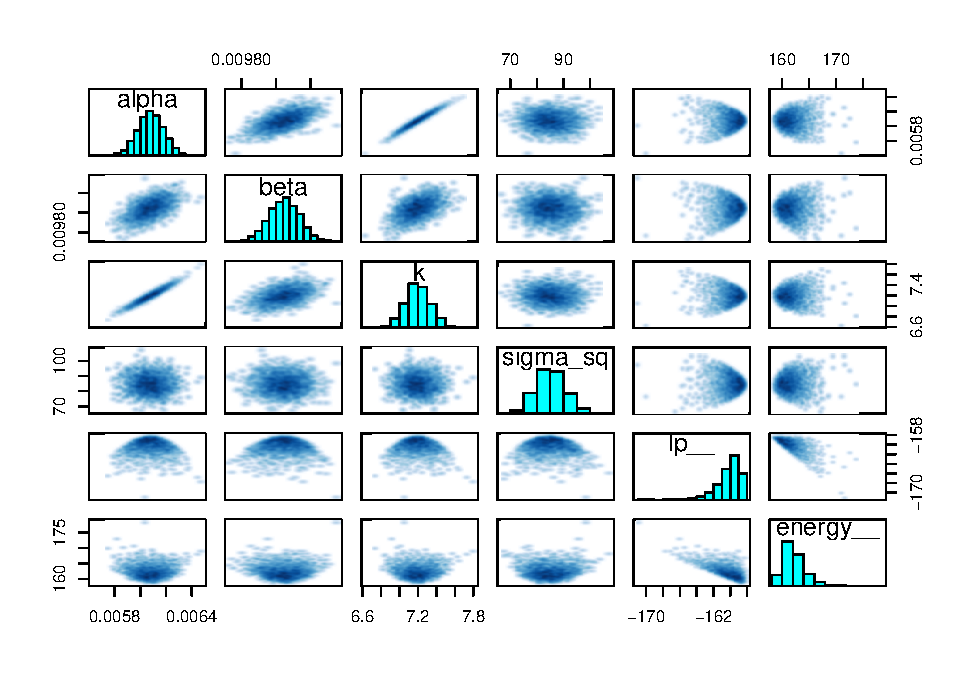
\includegraphics{multistep-model-comparison_files/figure-latex/model_beta-1.pdf}

\begin{Shaded}
\begin{Highlighting}[]
\NormalTok{H_BETA =}\StringTok{ }\KeywordTok{bridge_sampler}\NormalTok{(fit_beta)}
\end{Highlighting}
\end{Shaded}

\begin{verbatim}
## Iteration: 1
## Iteration: 2
## Iteration: 3
## Iteration: 4
## Iteration: 5
\end{verbatim}

\hypertarget{model-beta-sex}{%
\subsection{Model: Beta Sex}\label{model-beta-sex}}

\begin{verbatim}
## 
## CHECKING DATA AND PREPROCESSING FOR MODEL 'multistep_beta_sex' NOW.
## 
## COMPILING MODEL 'multistep_beta_sex' NOW.
## 
## STARTING SAMPLER FOR MODEL 'multistep_beta_sex' NOW.
\end{verbatim}

\begin{verbatim}
## Inference for Stan model: multistep_beta_sex.
## 4 chains, each with iter=2000; warmup=1000; thin=1; 
## post-warmup draws per chain=1000, total post-warmup draws=4000.
## 
##                mean se_mean   sd   2.5%    25%    50%    75%  97.5% n_eff Rhat
## alpha          8.51    0.01 0.19   8.11   8.40   8.52   8.64   8.85   662 1.00
## beta           0.01    0.00 0.00   0.01   0.01   0.01   0.01   0.01   635 1.00
## k             10.50    0.01 0.31   9.85  10.30  10.51  10.70  11.08   704 1.00
## alpha_sex     -0.20    0.01 0.24  -0.57  -0.38  -0.23  -0.05   0.35   699 1.01
## beta_sex       0.00    0.00 0.00   0.00   0.00   0.00   0.00   0.00   644 1.01
## k_sex          0.39    0.02 0.43  -0.29   0.08   0.34   0.65   1.34   762 1.00
## alpha_female   8.31    0.01 0.22   7.88   8.16   8.31   8.46   8.75  1149 1.00
## k_female      10.89    0.01 0.40  10.13  10.62  10.87  11.14  11.73  1167 1.00
## sigma_sq      11.15    0.09 3.39   5.99   8.66  10.68  13.03  19.20  1370 1.00
## lp__         -52.40    0.07 2.08 -57.28 -53.55 -52.06 -50.87 -49.38   836 1.00
## 
## Samples were drawn using NUTS(diag_e) at Thu Dec 17 10:16:12 2020.
## For each parameter, n_eff is a crude measure of effective sample size,
## and Rhat is the potential scale reduction factor on split chains (at 
## convergence, Rhat=1).
\end{verbatim}

\includegraphics{multistep-model-comparison_files/figure-latex/model_beta_sex-1.pdf}

\begin{verbatim}
## Warning: 14 of the 2000 log_prob() evaluations on the proposal draws produced
## -Inf/Inf.
\end{verbatim}

\begin{verbatim}
## Iteration: 1
## Iteration: 2
## Iteration: 3
## Iteration: 4
## Iteration: 5
## Iteration: 6
## Iteration: 7
## Iteration: 8
## Iteration: 9
## Iteration: 10
\end{verbatim}

\hypertarget{model-susceptibility}{%
\subsection{Model: Susceptibility}\label{model-susceptibility}}

\begin{Shaded}
\begin{Highlighting}[]
\CommentTok{# Lets try with nls to get an idea of parameter values to start with}

\NormalTok{nlm <-}\StringTok{ }\KeywordTok{nls}\NormalTok{(middle }\OperatorTok{~}\StringTok{ }\NormalTok{alpha}\OperatorTok{*}\NormalTok{agecut5_numeric}\OperatorTok{^}\NormalTok{(k}\DecValTok{-1}\NormalTok{)}\OperatorTok{*}\DecValTok{100000}\OperatorTok{/}\NormalTok{(}\DecValTok{1}\OperatorTok{+}\NormalTok{((}\DecValTok{1}\OperatorTok{-}\NormalTok{C)}\OperatorTok{/}\NormalTok{C)}\OperatorTok{*}\KeywordTok{exp}\NormalTok{(alpha}\OperatorTok{/}\NormalTok{k}\OperatorTok{*}\NormalTok{(agecut5_numeric}\OperatorTok{^}\NormalTok{k}\DecValTok{-1}\NormalTok{))), }\DataTypeTok{data=}\NormalTok{sim_df_ms_full,}\DataTypeTok{start=}\KeywordTok{list}\NormalTok{(}\DataTypeTok{alpha=}\FloatTok{1e-13}\NormalTok{, }\DataTypeTok{C=}\FloatTok{0.05}\NormalTok{, }\DataTypeTok{k=}\DecValTok{7}\NormalTok{))}

\KeywordTok{summary}\NormalTok{(nlm)}
\end{Highlighting}
\end{Shaded}

\begin{verbatim}
## 
## Formula: middle ~ alpha * agecut5_numeric^(k - 1) * 1e+05/(1 + ((1 - C)/C) * 
##     exp(alpha/k * (agecut5_numeric^k - 1)))
## 
## Parameters:
##        Estimate Std. Error t value Pr(>|t|)    
## alpha 1.200e-15  1.520e-15   0.789    0.445    
## C     8.024e-02  2.246e-03  35.729 1.48e-13 ***
## k     8.200e+00  2.920e-01  28.081 2.58e-12 ***
## ---
## Signif. codes:  0 '***' 0.001 '**' 0.01 '*' 0.05 '.' 0.1 ' ' 1
## 
## Residual standard error: 14 on 12 degrees of freedom
## 
## Number of iterations to convergence: 33 
## Achieved convergence tolerance: 2.017e-06
\end{verbatim}

\begin{Shaded}
\begin{Highlighting}[]
\NormalTok{mod_ms_suscept <-}\StringTok{ }\KeywordTok{stan_model}\NormalTok{(}\StringTok{'stan/multistep_susceptibility.stan'}\NormalTok{)}

\NormalTok{pars_suscept <-}\StringTok{ }\KeywordTok{c}\NormalTok{(}\StringTok{'alpha'}\NormalTok{,}\StringTok{'C'}\NormalTok{,}\StringTok{'k'}\NormalTok{,}\StringTok{'sigma_sq'}\NormalTok{)}

\NormalTok{data_list_suscept <-}\StringTok{ }\KeywordTok{list}\NormalTok{(}\DataTypeTok{C_prior_mean =} \DecValTok{5}\NormalTok{,}
                  \DataTypeTok{C_prior_sd =} \DecValTok{5}\NormalTok{,}
                  \DataTypeTok{alpha_prior_mean =} \DecValTok{0}\NormalTok{,}
                  \DataTypeTok{alpha_prior_sd =} \DecValTok{10}\NormalTok{,}
                  \DataTypeTok{k_prior_mean =} \DecValTok{7}\NormalTok{,}
                  \DataTypeTok{k_prior_sd =} \DecValTok{2}\NormalTok{,}
                  \DataTypeTok{N=}\KeywordTok{nrow}\NormalTok{(sim_df_ms_full),}
                  \DataTypeTok{x =}\NormalTok{ sim_df_ms_full}\OperatorTok{$}\NormalTok{agecut5_numeric,}
                  \DataTypeTok{y =}\NormalTok{ sim_df_ms_full}\OperatorTok{$}\NormalTok{middle,}
                  \DataTypeTok{y_min =}\NormalTok{ sim_df_ms_full}\OperatorTok{$}\NormalTok{lower,}
                  \DataTypeTok{y_max =}\NormalTok{ sim_df_ms_full}\OperatorTok{$}\NormalTok{upper)}

\NormalTok{init_suscept <-}\StringTok{ }\ControlFlowTok{function}\NormalTok{() \{}
  \KeywordTok{list}\NormalTok{(}\DataTypeTok{alpha =} \DecValTok{1}\NormalTok{, }\DataTypeTok{C =} \DecValTok{5}\NormalTok{, }\DataTypeTok{k =} \DecValTok{7}\NormalTok{, }\DataTypeTok{sigma_sq =} \DecValTok{80}\NormalTok{)}
\NormalTok{\}}


\NormalTok{fit_suscept <-}\StringTok{ }\KeywordTok{sampling}\NormalTok{(mod_ms_suscept, }\DataTypeTok{data =}\NormalTok{ data_list_suscept, }\DataTypeTok{seed =}\NormalTok{ SEED,}
                   \DataTypeTok{pars =}\NormalTok{ pars_suscept, }\DataTypeTok{chains =} \DecValTok{4}\NormalTok{, }\DataTypeTok{iter =} \DecValTok{2000}\NormalTok{, }
                   \DataTypeTok{init =}\NormalTok{ init_suscept,}
                   \DataTypeTok{control =} \KeywordTok{list}\NormalTok{(}\DataTypeTok{max_treedepth =} \DecValTok{15}\NormalTok{,}\DataTypeTok{adapt_delta=}\FloatTok{0.99}\NormalTok{),}
                   \DataTypeTok{verbose=}\OtherTok{TRUE}\NormalTok{)}
\end{Highlighting}
\end{Shaded}

\begin{verbatim}
## 
## CHECKING DATA AND PREPROCESSING FOR MODEL 'multistep_susceptibility' NOW.
## 
## COMPILING MODEL 'multistep_susceptibility' NOW.
## 
## STARTING SAMPLER FOR MODEL 'multistep_susceptibility' NOW.
\end{verbatim}

\begin{Shaded}
\begin{Highlighting}[]
\KeywordTok{print}\NormalTok{(fit_suscept)}
\end{Highlighting}
\end{Shaded}

\begin{verbatim}
## Inference for Stan model: multistep_susceptibility.
## 4 chains, each with iter=2000; warmup=1000; thin=1; 
## post-warmup draws per chain=1000, total post-warmup draws=4000.
## 
##            mean se_mean   sd   2.5%    25%    50%    75%  97.5% n_eff Rhat
## alpha      2.08    0.04 1.28   0.54   1.19   1.80   2.63   5.40  1072    1
## C          8.07    0.00 0.11   7.85   7.99   8.07   8.14   8.29  1305    1
## k          8.11    0.00 0.14   7.85   8.02   8.11   8.20   8.39  1078    1
## sigma_sq  45.03    0.13 5.41  35.21  41.25  44.81  48.57  55.78  1803    1
## lp__     -62.71    0.04 1.39 -66.24 -63.41 -62.40 -61.68 -60.92  1303    1
## 
## Samples were drawn using NUTS(diag_e) at Thu Dec 17 10:16:24 2020.
## For each parameter, n_eff is a crude measure of effective sample size,
## and Rhat is the potential scale reduction factor on split chains (at 
## convergence, Rhat=1).
\end{verbatim}

\begin{Shaded}
\begin{Highlighting}[]
\KeywordTok{summary}\NormalTok{(fit_suscept)}
\end{Highlighting}
\end{Shaded}

\begin{verbatim}
## $summary
##                mean     se_mean       sd        2.5%        25%        50%
## alpha      2.081815 0.039179839 1.282995   0.5392389   1.193651   1.795499
## C          8.067079 0.003020384 0.109130   7.8519989   7.993767   8.069164
## k          8.111873 0.004147213 0.136134   7.8527848   8.019597   8.107358
## sigma_sq  45.025049 0.127354703 5.408069  35.2095092  41.246230  44.805154
## lp__     -62.710318 0.038514858 1.390079 -66.2350004 -63.406137 -62.398196
##                 75%      97.5%    n_eff     Rhat
## alpha      2.628081   5.400695 1072.321 1.002264
## C          8.140125   8.287528 1305.463 1.003382
## k          8.201420   8.385170 1077.509 1.002887
## sigma_sq  48.569274  55.781604 1803.244 1.001258
## lp__     -61.679687 -60.924585 1302.635 1.000584
## 
## $c_summary
## , , chains = chain:1
## 
##           stats
## parameter        mean        sd       2.5%        25%        50%        75%
##   alpha      2.093684 1.3802858   0.538945   1.167477   1.797439   2.581022
##   C          8.067792 0.1142621   7.853162   7.990296   8.076368   8.144100
##   k          8.112822 0.1384938   7.840447   8.023220   8.106299   8.207138
##   sigma_sq  45.110722 5.3792350  35.395907  41.243943  44.965590  48.842416
##   lp__     -62.732627 1.3987597 -66.147000 -63.403521 -62.409392 -61.705184
##           stats
## parameter      97.5%
##   alpha      5.65894
##   C          8.29165
##   k          8.38381
##   sigma_sq  55.19920
##   lp__     -60.93106
## 
## , , chains = chain:2
## 
##           stats
## parameter        mean        sd       2.5%        25%        50%        75%
##   alpha      2.160689 1.3276493   0.544938   1.230762   1.790992   2.704708
##   C          8.074448 0.1060640   7.851939   8.010119   8.077895   8.140433
##   k          8.103344 0.1358151   7.839561   8.009751   8.106773   8.194770
##   sigma_sq  45.332280 5.5322662  35.073604  41.543817  44.938530  48.793776
##   lp__     -62.702747 1.4418870 -66.317680 -63.320017 -62.374462 -61.647994
##           stats
## parameter       97.5%
##   alpha      5.687106
##   C          8.290910
##   k          8.379733
##   sigma_sq  57.008280
##   lp__     -60.923386
## 
## , , chains = chain:3
## 
##           stats
## parameter        mean        sd        2.5%        25%        50%        75%
##   alpha      2.006148 1.2331694   0.5004308   1.130323   1.786528   2.556852
##   C          8.059005 0.1078391   7.8398162   7.987759   8.055518   8.130450
##   k          8.120893 0.1379884   7.8656126   8.027199   8.109833   8.211595
##   sigma_sq  45.077366 5.3460326  35.7464514  41.388825  44.687018  48.615211
##   lp__     -62.697360 1.3785139 -66.1448485 -63.402903 -62.398196 -61.669865
##           stats
## parameter       97.5%
##   alpha      5.185077
##   C          8.287246
##   k          8.402608
##   sigma_sq  56.182834
##   lp__     -60.923839
## 
## , , chains = chain:4
## 
##           stats
## parameter        mean        sd        2.5%        25%        50%        75%
##   alpha      2.066739 1.1782938   0.5772255   1.206438   1.806812   2.666874
##   C          8.067071 0.1077890   7.8593262   7.994097   8.068732   8.143767
##   k          8.110431 0.1317621   7.8701392   8.016866   8.105328   8.196396
##   sigma_sq  44.579827 5.3527057  35.0301881  40.844941  44.399325  48.130723
##   lp__     -62.708537 1.3410786 -65.9537491 -63.435713 -62.409365 -61.698327
##           stats
## parameter       97.5%
##   alpha      4.926724
##   C          8.269402
##   k          8.370048
##   sigma_sq  55.019893
##   lp__     -60.927572
\end{verbatim}

\begin{Shaded}
\begin{Highlighting}[]
\KeywordTok{pairs}\NormalTok{(fit_suscept,}\DataTypeTok{pars=}\NormalTok{pars_suscept)}
\end{Highlighting}
\end{Shaded}

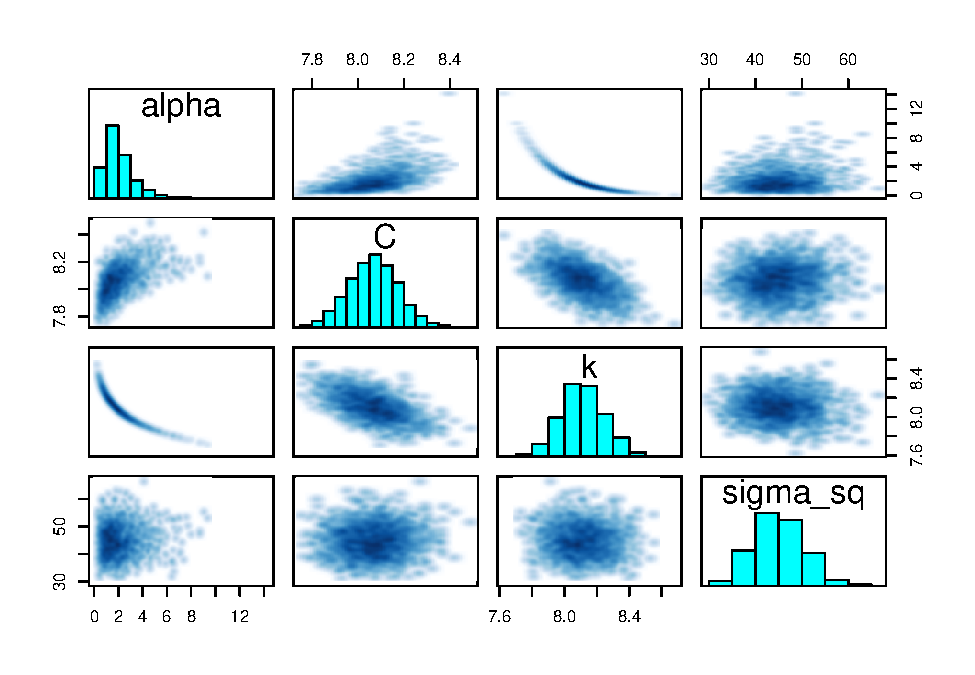
\includegraphics{multistep-model-comparison_files/figure-latex/model_susceptibility-1.pdf}

\begin{Shaded}
\begin{Highlighting}[]
\NormalTok{H_SUSCEPT =}\StringTok{ }\KeywordTok{bridge_sampler}\NormalTok{(fit_suscept)}
\end{Highlighting}
\end{Shaded}

\begin{verbatim}
## Iteration: 1
## Iteration: 2
## Iteration: 3
## Iteration: 4
## Iteration: 5
## Iteration: 6
## Iteration: 7
\end{verbatim}

\begin{Shaded}
\begin{Highlighting}[]
\KeywordTok{bf}\NormalTok{(H_SUSCEPT,H_AD)}
\end{Highlighting}
\end{Shaded}

\begin{verbatim}
## Estimated Bayes factor in favor of H_SUSCEPT over H_AD: 0.00000
\end{verbatim}

\begin{Shaded}
\begin{Highlighting}[]
\KeywordTok{bf}\NormalTok{(H_BETA,H_AD)}
\end{Highlighting}
\end{Shaded}

\begin{verbatim}
## Estimated Bayes factor in favor of H_BETA over H_AD: 0.00000
\end{verbatim}

\begin{Shaded}
\begin{Highlighting}[]
\KeywordTok{bf}\NormalTok{(H_SUSCEPT,H_BETA)}
\end{Highlighting}
\end{Shaded}

\begin{verbatim}
## Estimated Bayes factor in favor of H_SUSCEPT over H_BETA: 100685273026986911994395880325120.00000
\end{verbatim}

\hypertarget{model-susceptibility-fixed-c}{%
\subsection{Model: Susceptibility fixed
C}\label{model-susceptibility-fixed-c}}

\begin{Shaded}
\begin{Highlighting}[]
\CommentTok{# Iterate over values of C, to see how plausible alterative values of C are}

\NormalTok{mod_ms_suscept_fixed <-}\StringTok{ }\KeywordTok{stan_model}\NormalTok{(}\StringTok{'stan/multistep_susceptibility_fixed_C.stan'}\NormalTok{)}

\NormalTok{pars_suscept_fixed <-}\StringTok{ }\KeywordTok{c}\NormalTok{(}\StringTok{'alpha'}\NormalTok{,}\StringTok{'k'}\NormalTok{,}\StringTok{'sigma_sq'}\NormalTok{)}

\NormalTok{data_list_suscept_fixed <-}\StringTok{ }\KeywordTok{list}\NormalTok{(}\DataTypeTok{C =} \DecValTok{3}\NormalTok{,}
                  \DataTypeTok{alpha_prior_mean =} \DecValTok{0}\NormalTok{,}
                  \DataTypeTok{alpha_prior_sd =} \DecValTok{10}\NormalTok{,}
                  \DataTypeTok{k_prior_mean =} \DecValTok{7}\NormalTok{,}
                  \DataTypeTok{k_prior_sd =} \DecValTok{2}\NormalTok{,}
                  \DataTypeTok{N=}\KeywordTok{nrow}\NormalTok{(sim_df_ms_full),}
                  \DataTypeTok{x =}\NormalTok{ sim_df_ms_full}\OperatorTok{$}\NormalTok{agecut5_numeric,}
                  \DataTypeTok{y =}\NormalTok{ sim_df_ms_full}\OperatorTok{$}\NormalTok{middle,}
                  \DataTypeTok{y_min =}\NormalTok{ sim_df_ms_full}\OperatorTok{$}\NormalTok{lower,}
                  \DataTypeTok{y_max =}\NormalTok{ sim_df_ms_full}\OperatorTok{$}\NormalTok{upper)}

\NormalTok{init_suscept_fixed <-}\StringTok{ }\ControlFlowTok{function}\NormalTok{() \{}
  \KeywordTok{list}\NormalTok{(}\DataTypeTok{alpha =} \DecValTok{1}\NormalTok{, }\DataTypeTok{k =} \DecValTok{7}\NormalTok{, }\DataTypeTok{sigma_sq =} \DecValTok{80}\NormalTok{)}
\NormalTok{\}}

\NormalTok{fit_suscept_fixed <-}\StringTok{ }\KeywordTok{sampling}\NormalTok{(mod_ms_suscept_fixed, }
                              \DataTypeTok{data =}\NormalTok{ data_list_suscept_fixed, }
                              \DataTypeTok{seed =}\NormalTok{ SEED,}
                              \DataTypeTok{pars =}\NormalTok{ pars_suscept_fixed, }
                              \DataTypeTok{chains =} \DecValTok{4}\NormalTok{, }\DataTypeTok{iter =} \DecValTok{2000}\NormalTok{, }
                              \DataTypeTok{init =}\NormalTok{ init_suscept_fixed,}
                              \DataTypeTok{control =} \KeywordTok{list}\NormalTok{(}\DataTypeTok{max_treedepth =} \DecValTok{15}\NormalTok{,}
                                             \DataTypeTok{adapt_delta=}\FloatTok{0.99}\NormalTok{),}
                              \DataTypeTok{verbose=}\OtherTok{TRUE}\NormalTok{)}
\end{Highlighting}
\end{Shaded}

\begin{verbatim}
## 
## CHECKING DATA AND PREPROCESSING FOR MODEL 'multistep_susceptibility_fixed_C' NOW.
## 
## COMPILING MODEL 'multistep_susceptibility_fixed_C' NOW.
## 
## STARTING SAMPLER FOR MODEL 'multistep_susceptibility_fixed_C' NOW.
\end{verbatim}

\begin{Shaded}
\begin{Highlighting}[]
\NormalTok{H_SUSCEPT_FIXED =}\StringTok{ }\KeywordTok{bridge_sampler}\NormalTok{(fit_suscept_fixed)}
\end{Highlighting}
\end{Shaded}

\begin{verbatim}
## Iteration: 1
## Iteration: 2
## Iteration: 3
## Iteration: 4
## Iteration: 5
## Iteration: 6
## Iteration: 7
## Iteration: 8
## Iteration: 9
## Iteration: 10
## Iteration: 11
## Iteration: 12
## Iteration: 13
## Iteration: 14
\end{verbatim}

\begin{Shaded}
\begin{Highlighting}[]
\KeywordTok{bf}\NormalTok{(H_SUSCEPT_FIXED,H_AD)}
\end{Highlighting}
\end{Shaded}

\begin{verbatim}
## Estimated Bayes factor in favor of H_SUSCEPT_FIXED over H_AD: 0.00000
\end{verbatim}

\hypertarget{model-susceptibility-sex}{%
\subsection{Model: Susceptibility Sex}\label{model-susceptibility-sex}}

\begin{Shaded}
\begin{Highlighting}[]
\NormalTok{mod_ms_suscept_sex <-}\StringTok{ }\KeywordTok{stan_model}\NormalTok{(}\StringTok{'stan/multistep_susceptibility_sex.stan'}\NormalTok{)}

\NormalTok{pars_suscept_sex <-}\StringTok{ }\KeywordTok{c}\NormalTok{(}\StringTok{'alpha'}\NormalTok{,}\StringTok{'C'}\NormalTok{,}\StringTok{'k'}\NormalTok{,}
                      \StringTok{'alpha_sex'}\NormalTok{,}\StringTok{'C_sex'}\NormalTok{,}\StringTok{'k_sex'}\NormalTok{,}
                      \StringTok{'alpha_female'}\NormalTok{,}\StringTok{'C_female'}\NormalTok{,}\StringTok{'k_female'}\NormalTok{,}\StringTok{'sigma_sq'}\NormalTok{)}

\NormalTok{data_list_suscept_sex <-}\StringTok{ }\KeywordTok{list}\NormalTok{(}\DataTypeTok{C_prior_mean =} \DecValTok{5}\NormalTok{,}
                  \DataTypeTok{C_prior_sd =} \DecValTok{5}\NormalTok{,}
                  \DataTypeTok{alpha_prior_mean =} \DecValTok{0}\NormalTok{,}
                  \DataTypeTok{alpha_prior_sd =} \DecValTok{10}\NormalTok{,}
                  \DataTypeTok{k_prior_mean =} \DecValTok{7}\NormalTok{,}
                  \DataTypeTok{k_prior_sd =} \DecValTok{2}\NormalTok{,}
                  \DataTypeTok{N=}\KeywordTok{nrow}\NormalTok{(sim_df_ms_sex_full),}
                  \DataTypeTok{DEBUG=}\DecValTok{0}\NormalTok{,}
                  \DataTypeTok{x =}\NormalTok{ sim_df_ms_sex_full}\OperatorTok{$}\NormalTok{agecut5_numeric,}
                  \DataTypeTok{y =}\NormalTok{ sim_df_ms_sex_full}\OperatorTok{$}\NormalTok{middle,}
                  \DataTypeTok{sex =} \KeywordTok{abs}\NormalTok{(}\KeywordTok{as.numeric}\NormalTok{(}\KeywordTok{factor}\NormalTok{(sim_df_ms_sex_full}\OperatorTok{$}\NormalTok{sex))}\OperatorTok{-}\DecValTok{1}\NormalTok{),}
                  \DataTypeTok{y_min =}\NormalTok{ sim_df_ms_sex_full}\OperatorTok{$}\NormalTok{lower,}
                  \DataTypeTok{y_max =}\NormalTok{ sim_df_ms_sex_full}\OperatorTok{$}\NormalTok{upper)}

\NormalTok{init_ms_suspect_sex <-}\StringTok{ }\ControlFlowTok{function}\NormalTok{() \{}
  \KeywordTok{list}\NormalTok{(}\DataTypeTok{alpha =} \DecValTok{2}\NormalTok{, }\DataTypeTok{C =} \DecValTok{8}\NormalTok{, }\DataTypeTok{k =} \DecValTok{8}\NormalTok{, }\DataTypeTok{alpha_sex=}\DecValTok{0}\NormalTok{, }\DataTypeTok{C_sex=}\DecValTok{0}\NormalTok{, }\DataTypeTok{k_sex=}\DecValTok{0}\NormalTok{, }\DataTypeTok{sigma_sq =} \DecValTok{80}\NormalTok{)}
\NormalTok{\}}

\NormalTok{fit_suscept_sex <-}\StringTok{ }\KeywordTok{sampling}\NormalTok{(mod_ms_suscept_sex, }\DataTypeTok{data =}\NormalTok{ data_list_suscept_sex, }
                            \DataTypeTok{seed =}\NormalTok{ SEED, }\DataTypeTok{init =}\NormalTok{ init_ms_suspect_sex,}
                   \DataTypeTok{pars =}\NormalTok{ pars_suscept_sex, }\DataTypeTok{chains =} \DecValTok{4}\NormalTok{, }\DataTypeTok{iter =} \DecValTok{2000}\NormalTok{,}
                   \DataTypeTok{control =} \KeywordTok{list}\NormalTok{(}\DataTypeTok{max_treedepth =} \DecValTok{15}\NormalTok{,}\DataTypeTok{adapt_delta=}\FloatTok{0.99}\NormalTok{),}
                   \DataTypeTok{verbose=}\OtherTok{TRUE}\NormalTok{)}
\end{Highlighting}
\end{Shaded}

\begin{verbatim}
## 
## CHECKING DATA AND PREPROCESSING FOR MODEL 'multistep_susceptibility_sex' NOW.
## 
## COMPILING MODEL 'multistep_susceptibility_sex' NOW.
## 
## STARTING SAMPLER FOR MODEL 'multistep_susceptibility_sex' NOW.
\end{verbatim}

\begin{verbatim}
## Warning: There were 12 divergent transitions after warmup. Increasing adapt_delta above 0.99 may help. See
## http://mc-stan.org/misc/warnings.html#divergent-transitions-after-warmup
\end{verbatim}

\begin{verbatim}
## Warning: Examine the pairs() plot to diagnose sampling problems
\end{verbatim}

\begin{Shaded}
\begin{Highlighting}[]
\KeywordTok{print}\NormalTok{(fit_suscept_sex)}
\end{Highlighting}
\end{Shaded}

\begin{verbatim}
## Inference for Stan model: multistep_susceptibility_sex.
## 4 chains, each with iter=2000; warmup=1000; thin=1; 
## post-warmup draws per chain=1000, total post-warmup draws=4000.
## 
##                 mean se_mean   sd    2.5%     25%     50%     75%   97.5% n_eff
## alpha           9.94    0.13 3.85    3.86    7.15    9.48   12.28   18.58   922
## C              11.19    0.00 0.14   10.92   11.10   11.19   11.28   11.45  1403
## k               7.70    0.00 0.09    7.54    7.63    7.69    7.76    7.90   963
## alpha_sex      -5.50    0.19 5.29  -15.36   -8.75   -5.72   -2.55    6.31   802
## C_sex          -4.82    0.01 0.19   -5.20   -4.95   -4.82   -4.70   -4.43  1341
## k_sex           0.28    0.01 0.22   -0.13    0.12    0.28    0.43    0.73   876
## alpha_female    4.44    0.14 4.26    0.49    1.54    3.01    5.95   16.23   962
## C_female        6.36    0.00 0.14    6.09    6.27    6.37    6.46    6.64  1957
## k_female        7.98    0.01 0.21    7.59    7.82    7.98    8.13    8.40  1026
## sigma_sq       83.32    0.12 5.62   72.70   79.48   83.11   87.14   94.80  2217
## lp__         -181.94    0.07 2.02 -186.80 -183.10 -181.65 -180.42 -178.99   933
##              Rhat
## alpha        1.00
## C            1.01
## k            1.01
## alpha_sex    1.01
## C_sex        1.01
## k_sex        1.00
## alpha_female 1.00
## C_female     1.00
## k_female     1.00
## sigma_sq     1.00
## lp__         1.00
## 
## Samples were drawn using NUTS(diag_e) at Thu Dec 17 10:17:20 2020.
## For each parameter, n_eff is a crude measure of effective sample size,
## and Rhat is the potential scale reduction factor on split chains (at 
## convergence, Rhat=1).
\end{verbatim}

\begin{Shaded}
\begin{Highlighting}[]
\KeywordTok{pairs}\NormalTok{(fit_suscept_sex,}\DataTypeTok{pars=}\KeywordTok{c}\NormalTok{(}\StringTok{"C"}\NormalTok{,}\StringTok{"k"}\NormalTok{,}\StringTok{"alpha"}\NormalTok{,}\StringTok{"C_sex"}\NormalTok{,}\StringTok{"k_sex"}\NormalTok{,}\StringTok{"alpha_sex"}\NormalTok{))}
\end{Highlighting}
\end{Shaded}

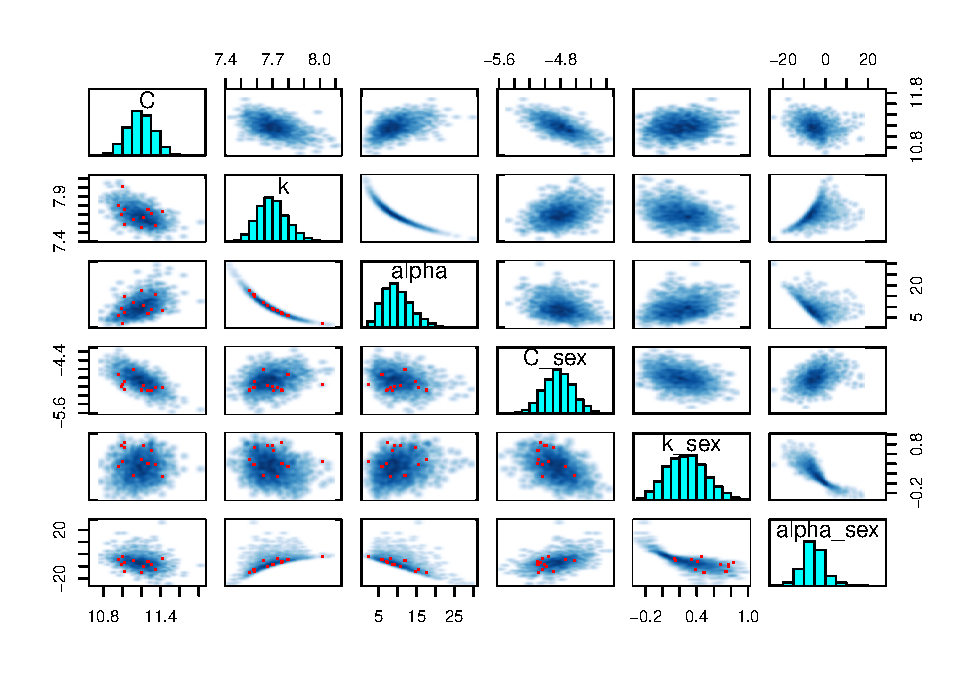
\includegraphics{multistep-model-comparison_files/figure-latex/model_susceptibility_sex-1.pdf}

\begin{Shaded}
\begin{Highlighting}[]
\CommentTok{## Run in console}
\KeywordTok{pdf}\NormalTok{(}\StringTok{"plots/suscept_sex_pairs_diagnosis.pdf"}\NormalTok{)}
\KeywordTok{pairs}\NormalTok{(fit_suscept_sex,}\DataTypeTok{pars=}\KeywordTok{c}\NormalTok{(}\StringTok{"C"}\NormalTok{,}\StringTok{"k"}\NormalTok{,}\StringTok{"alpha"}\NormalTok{,}\StringTok{"C_sex"}\NormalTok{,}\StringTok{"k_sex"}\NormalTok{,}\StringTok{"alpha_sex"}\NormalTok{))}
\KeywordTok{dev.off}\NormalTok{()}
\end{Highlighting}
\end{Shaded}

\begin{verbatim}
## pdf 
##   2
\end{verbatim}

\begin{Shaded}
\begin{Highlighting}[]
\CommentTok{#H_SUSCEPT = bridge_sampler(fit_suscept)}

\CommentTok{#bf(H_SUSCEPT,H_AD)}
\CommentTok{#bf(H_BETA,H_AD)}
\CommentTok{#bf(H_SUSCEPT,H_BETA)}
\end{Highlighting}
\end{Shaded}

\hypertarget{plot-age-specific-incidence-non-log}{%
\subsection{Plot: Age-specific incidence
non-log}\label{plot-age-specific-incidence-non-log}}

\begin{Shaded}
\begin{Highlighting}[]
\NormalTok{fig2_age_specific_incidence <-}\StringTok{ }\NormalTok{sim_df_ms_full }\OperatorTok
\StringTok{  }\KeywordTok{ggplot}\NormalTok{(}\KeywordTok{aes}\NormalTok{(}\DataTypeTok{x=}\NormalTok{agecut5,}\DataTypeTok{y=}\NormalTok{middle,}\DataTypeTok{group=}\StringTok{"incidence"}\NormalTok{))}\OperatorTok{+}
\StringTok{  }\KeywordTok{geom_ribbon}\NormalTok{(}\KeywordTok{aes}\NormalTok{(}\DataTypeTok{ymin=}\NormalTok{lower,}\DataTypeTok{ymax=}\NormalTok{upper),}\DataTypeTok{alpha=}\FloatTok{0.3}\NormalTok{)}\OperatorTok{+}
\StringTok{  }\KeywordTok{scale_x_discrete}\NormalTok{(}\StringTok{"Age"}\NormalTok{, }\DataTypeTok{labels =} \KeywordTok{c}\NormalTok{(}\StringTok{"30"}\NormalTok{,}\StringTok{""}\NormalTok{,}
                                     \StringTok{"40"}\NormalTok{,}\StringTok{""}\NormalTok{,}\StringTok{"50"}\NormalTok{,}\StringTok{""}\NormalTok{,}
                                     \StringTok{"60"}\NormalTok{,}\StringTok{""}\NormalTok{,}\StringTok{"70"}\NormalTok{,}\StringTok{""}\NormalTok{,}
                                     \StringTok{"80"}\NormalTok{,}\StringTok{""}\NormalTok{,}\StringTok{"90"}\NormalTok{,}\StringTok{""}\NormalTok{,}
                                     \StringTok{"100+"}
\NormalTok{  ))}\OperatorTok{+}
\StringTok{  }\KeywordTok{geom_line}\NormalTok{(}\DataTypeTok{size=}\FloatTok{0.2}\NormalTok{)}\OperatorTok{+}\KeywordTok{geom_point}\NormalTok{(}\DataTypeTok{size=}\DecValTok{2}\NormalTok{,}\DataTypeTok{fill=}\StringTok{"grey"}\NormalTok{)}\OperatorTok{+}
\StringTok{  }\KeywordTok{ylab}\NormalTok{(}\StringTok{"Incidence}\CharTok{\textbackslash{}n}\StringTok{(per 100 000 per year)"}\NormalTok{)}\OperatorTok{+}
\StringTok{  }\KeywordTok{scale_shape_manual}\NormalTok{(}\DataTypeTok{values=}\KeywordTok{c}\NormalTok{(}\DecValTok{21}\NormalTok{))}\OperatorTok{+}
\StringTok{  }\KeywordTok{xlab}\NormalTok{(}\StringTok{"Age"}\NormalTok{)}\OperatorTok{+}\StringTok{ }\KeywordTok{theme}\NormalTok{(}\DataTypeTok{legend.position =} \StringTok{"none"}\NormalTok{)}\OperatorTok{+}
\StringTok{  }\KeywordTok{annotate}\NormalTok{(}\StringTok{"text"}\NormalTok{,}\DataTypeTok{x=}\DecValTok{1}\NormalTok{,}\DataTypeTok{y=}\DecValTok{300}\NormalTok{,}\DataTypeTok{label=}\StringTok{"A"}\NormalTok{)}

\KeywordTok{plot}\NormalTok{(fig2_age_specific_incidence)}
\end{Highlighting}
\end{Shaded}

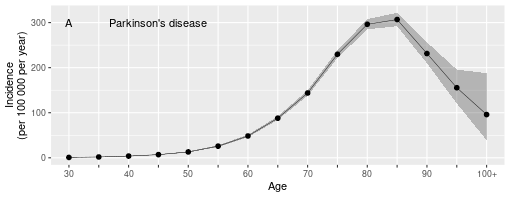
\includegraphics{multistep-model-comparison_files/figure-latex/age-specific-incidence-figure-1.png}

\begin{Shaded}
\begin{Highlighting}[]
\KeywordTok{ggsave}\NormalTok{(}\StringTok{"plots/multistep-incidence-by-age.pdf"}\NormalTok{,}\DataTypeTok{width=}\DecValTok{5}\NormalTok{,}\DataTypeTok{height=}\DecValTok{3}\NormalTok{)}
\KeywordTok{ggsave}\NormalTok{(}\StringTok{"plots/multistep-incidence-by-age.png"}\NormalTok{,}\DataTypeTok{width=}\DecValTok{5}\NormalTok{,}\DataTypeTok{height=}\DecValTok{3}\NormalTok{)}
\end{Highlighting}
\end{Shaded}

\hypertarget{plot-age-specific-incidence-by-sex-non-log}{%
\subsection{Plot: Age-specific incidence by sex
non-log}\label{plot-age-specific-incidence-by-sex-non-log}}

\begin{Shaded}
\begin{Highlighting}[]
\NormalTok{fig2_age_sex_specific_incidence <-}\StringTok{ }\NormalTok{sim_df_ms_sex_full }\OperatorTok
\StringTok{  }\KeywordTok{ggplot}\NormalTok{(}\KeywordTok{aes}\NormalTok{(}\DataTypeTok{x=}\NormalTok{agecut5,}\DataTypeTok{y=}\NormalTok{middle,}\DataTypeTok{colour=}\NormalTok{sex,}\DataTypeTok{group=}\NormalTok{sex,}\DataTypeTok{shape=}\NormalTok{sex))}\OperatorTok{+}
\StringTok{  }\KeywordTok{geom_errorbar}\NormalTok{(}\KeywordTok{aes}\NormalTok{(}\DataTypeTok{ymin=}\NormalTok{lower,}\DataTypeTok{ymax=}\NormalTok{upper), }\DataTypeTok{width=}\DecValTok{0}\NormalTok{)}\OperatorTok{+}
\StringTok{  }\KeywordTok{scale_x_discrete}\NormalTok{(}\StringTok{"Age"}\NormalTok{, }\DataTypeTok{labels =} \KeywordTok{c}\NormalTok{(}\StringTok{"30"}\NormalTok{,}\StringTok{""}\NormalTok{,}
                                     \StringTok{"40"}\NormalTok{,}\StringTok{""}\NormalTok{,}\StringTok{"50"}\NormalTok{,}\StringTok{""}\NormalTok{,}
                                     \StringTok{"60"}\NormalTok{,}\StringTok{""}\NormalTok{,}\StringTok{"70"}\NormalTok{,}\StringTok{""}\NormalTok{,}
                                     \StringTok{"80"}\NormalTok{,}\StringTok{""}\NormalTok{,}\StringTok{"90"}\NormalTok{,}\StringTok{""}\NormalTok{,}
                                     \StringTok{"100+"}
\NormalTok{  ))}\OperatorTok{+}
\StringTok{  }\KeywordTok{geom_line}\NormalTok{(}\DataTypeTok{size=}\FloatTok{0.2}\NormalTok{)}\OperatorTok{+}\KeywordTok{geom_point}\NormalTok{(}\DataTypeTok{size=}\DecValTok{2}\NormalTok{,}\DataTypeTok{fill=}\StringTok{"grey"}\NormalTok{)}\OperatorTok{+}
\StringTok{  }\KeywordTok{ylab}\NormalTok{(}\StringTok{"Incidence}\CharTok{\textbackslash{}n}\StringTok{(per 100 000 per year)"}\NormalTok{)}\OperatorTok{+}
\StringTok{  }\CommentTok{#scale_shape_manual(values=c(21))+}
\StringTok{  }\KeywordTok{scale_color_manual}\NormalTok{(}\DataTypeTok{values =}\NormalTok{ colours_mf)}\OperatorTok{+}
\StringTok{  }\KeywordTok{xlab}\NormalTok{(}\StringTok{"Age"}\NormalTok{) }\OperatorTok{+}\StringTok{ }
\StringTok{  }\KeywordTok{theme}\NormalTok{(}\DataTypeTok{legend.position =} \KeywordTok{c}\NormalTok{(}\FloatTok{0.3}\NormalTok{,}\FloatTok{0.7}\NormalTok{),}
                         \DataTypeTok{legend.title =} \KeywordTok{element_blank}\NormalTok{()) }\OperatorTok{+}
\StringTok{  }\KeywordTok{annotate}\NormalTok{(}\StringTok{"text"}\NormalTok{,}\DataTypeTok{x=}\DecValTok{1}\NormalTok{,}\DataTypeTok{y=}\DecValTok{450}\NormalTok{,}\DataTypeTok{label=}\StringTok{"D"}\NormalTok{)}

\KeywordTok{plot}\NormalTok{(fig2_age_sex_specific_incidence)}
\end{Highlighting}
\end{Shaded}

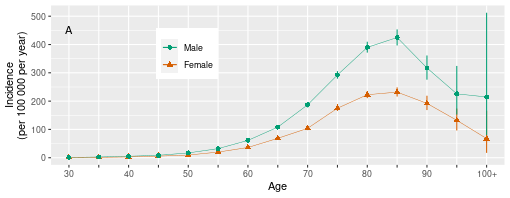
\includegraphics{multistep-model-comparison_files/figure-latex/age-sex-specific-incidence-figure-1.png}

\begin{Shaded}
\begin{Highlighting}[]
\KeywordTok{ggsave}\NormalTok{(}\StringTok{"plots/multistep-incidence-by-sex-age.pdf"}\NormalTok{,}\DataTypeTok{width=}\DecValTok{5}\NormalTok{,}\DataTypeTok{height=}\DecValTok{3}\NormalTok{)}
\KeywordTok{ggsave}\NormalTok{(}\StringTok{"plots/multistep-incidence-by-sex-age.png"}\NormalTok{,}\DataTypeTok{width=}\DecValTok{5}\NormalTok{,}\DataTypeTok{height=}\DecValTok{3}\NormalTok{)}
\end{Highlighting}
\end{Shaded}

\hypertarget{plot-linear-model}{%
\subsection{Plot: Linear model}\label{plot-linear-model}}

\begin{Shaded}
\begin{Highlighting}[]
\CommentTok{# Extract fitted values from model}
\NormalTok{values_l =}\StringTok{ }\KeywordTok{summary}\NormalTok{(fit_linear)}\OperatorTok{$}\NormalTok{summary}

\NormalTok{start=}\FloatTok{0.0}
\NormalTok{end =}\StringTok{ }\KeywordTok{max}\NormalTok{(sim_df_ms_model}\OperatorTok{$}\NormalTok{agecut5_scaled)}
\NormalTok{m =}\StringTok{ }\NormalTok{values_l[}\DecValTok{1}\NormalTok{,}\DecValTok{1}\NormalTok{]}
\NormalTok{c =}\StringTok{ }\NormalTok{values_l[}\DecValTok{2}\NormalTok{,}\DecValTok{1}\NormalTok{]}



\NormalTok{fig2_log_linear <-}\StringTok{ }\NormalTok{sim_df_ms_full }\OperatorTok
\StringTok{  }\KeywordTok{ggplot}\NormalTok{(}\KeywordTok{aes}\NormalTok{(}\DataTypeTok{x=}\NormalTok{agecut5_scaled,}\DataTypeTok{y=}\NormalTok{middle_log,}
             \DataTypeTok{group=}\NormalTok{type,}\DataTypeTok{colour=}\NormalTok{restriction))}\OperatorTok{+}
\StringTok{  }\KeywordTok{geom_errorbar}\NormalTok{(}\KeywordTok{aes}\NormalTok{(}\DataTypeTok{ymin=}\NormalTok{lower_log,}\DataTypeTok{ymax=}\NormalTok{upper_log), }\DataTypeTok{width=}\DecValTok{0}\NormalTok{)}\OperatorTok{+}
\StringTok{  }\KeywordTok{ylab}\NormalTok{(}\StringTok{"Log Incidence}\CharTok{\textbackslash{}n}\StringTok{(per 100 000 per year)"}\NormalTok{) }\OperatorTok{+}
\StringTok{  }\KeywordTok{xlab}\NormalTok{(}\StringTok{"log(Age) - log(30)"}\NormalTok{) }\OperatorTok{+}\StringTok{ }
\StringTok{  }\KeywordTok{theme}\NormalTok{(}\DataTypeTok{legend.position =} \StringTok{"none"}\NormalTok{) }\OperatorTok{+}
\StringTok{  }\KeywordTok{geom_segment}\NormalTok{(}\DataTypeTok{x=}\NormalTok{start,}\DataTypeTok{y=}\NormalTok{c}\OperatorTok{+}\NormalTok{m}\OperatorTok{*}\NormalTok{start,}
               \DataTypeTok{xend=}\NormalTok{end,}\DataTypeTok{yend=}\NormalTok{c}\OperatorTok{+}\NormalTok{m}\OperatorTok{*}\NormalTok{end,}\DataTypeTok{colour=}\StringTok{"#CC79A7"}\NormalTok{)}\OperatorTok{+}
\StringTok{  }\KeywordTok{geom_point}\NormalTok{(}\DataTypeTok{size=}\DecValTok{2}\NormalTok{) }\OperatorTok{+}
\StringTok{  }\KeywordTok{scale_colour_manual}\NormalTok{(}\DataTypeTok{values =}\NormalTok{ colours_modelled)}\OperatorTok{+}
\StringTok{  }\KeywordTok{annotate}\NormalTok{(}\StringTok{"text"}\NormalTok{,}\DataTypeTok{x=}\DecValTok{0}\NormalTok{,}\DataTypeTok{y=}\DecValTok{5}\NormalTok{,}\DataTypeTok{label=}\StringTok{"B"}\NormalTok{)}

\KeywordTok{plot}\NormalTok{(fig2_log_linear)}
\end{Highlighting}
\end{Shaded}

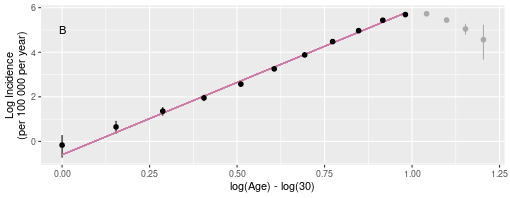
\includegraphics{multistep-model-comparison_files/figure-latex/linear-figure-1.png}

\begin{Shaded}
\begin{Highlighting}[]
\KeywordTok{ggsave}\NormalTok{(}\StringTok{"plots/multistep-log-relationship.pdf"}\NormalTok{,}\DataTypeTok{width=}\DecValTok{6}\NormalTok{,}\DataTypeTok{height=}\DecValTok{4}\NormalTok{)}
\KeywordTok{ggsave}\NormalTok{(}\StringTok{"plots/multistep-log-relationship.png"}\NormalTok{,}\DataTypeTok{width=}\DecValTok{6}\NormalTok{,}\DataTypeTok{height=}\DecValTok{4}\NormalTok{)}
\end{Highlighting}
\end{Shaded}

\hypertarget{plot-broken-stick-model}{%
\subsection{Plot: Broken-stick model}\label{plot-broken-stick-model}}

\begin{Shaded}
\begin{Highlighting}[]
\CommentTok{# Extract fitted values from model}
\NormalTok{values_bs =}\StringTok{ }\KeywordTok{summary}\NormalTok{(fit_bs)}\OperatorTok{$}\NormalTok{summary}

\NormalTok{m_early=values_bs[}\DecValTok{1}\NormalTok{,}\DecValTok{1}\NormalTok{]}
\NormalTok{m_late=values_bs[}\DecValTok{2}\NormalTok{,}\DecValTok{1}\NormalTok{]}
\NormalTok{bp=values_bs[}\DecValTok{3}\NormalTok{,}\DecValTok{1}\NormalTok{]}
\NormalTok{c=values_bs[}\DecValTok{4}\NormalTok{,}\DecValTok{1}\NormalTok{]}

\NormalTok{offset =}\StringTok{ }\FloatTok{0.25}

\NormalTok{x1 =}\StringTok{ }\NormalTok{start}
\NormalTok{y1 =}\StringTok{ }\NormalTok{c}\OperatorTok{+}\NormalTok{m_early}\OperatorTok{*}\NormalTok{x1}

\NormalTok{x2 =}\StringTok{ }\NormalTok{bp}
\NormalTok{y2 =}\StringTok{ }\NormalTok{c}\OperatorTok{+}\NormalTok{m_early}\OperatorTok{*}\NormalTok{x2}

\CommentTok{#x2a = bp+offset}
\CommentTok{#y2a = c+m_early*x2a}

\NormalTok{x2a =}\StringTok{ }\NormalTok{end}
\NormalTok{y2a =}\StringTok{ }\NormalTok{c}\OperatorTok{+}\NormalTok{m_early}\OperatorTok{*}\NormalTok{x2a}

\CommentTok{#x2b = bp-offset}
\CommentTok{#y2b = y2-m_late*offset}

\NormalTok{x2b =}\StringTok{ }\NormalTok{start}
\NormalTok{y2b =}\StringTok{ }\NormalTok{y2}\OperatorTok{-}\NormalTok{m_late}\OperatorTok{*}\NormalTok{(bp}\OperatorTok{-}\NormalTok{start)}

\NormalTok{x3 =}\StringTok{ }\NormalTok{end}
\NormalTok{y3 =}\StringTok{ }\NormalTok{y2}\OperatorTok{+}\NormalTok{(end}\OperatorTok{-}\NormalTok{bp)}\OperatorTok{*}\NormalTok{m_late}

\NormalTok{fig2_log_broken_stick <-}\StringTok{ }\NormalTok{sim_df_ms_full }\OperatorTok
\StringTok{  }\KeywordTok{ggplot}\NormalTok{(}\KeywordTok{aes}\NormalTok{(}\DataTypeTok{x=}\NormalTok{agecut5_scaled,}\DataTypeTok{y=}\NormalTok{middle_log,}
             \DataTypeTok{group=}\NormalTok{type,}\DataTypeTok{colour=}\NormalTok{restriction))}\OperatorTok{+}
\StringTok{  }\KeywordTok{geom_errorbar}\NormalTok{(}\KeywordTok{aes}\NormalTok{(}\DataTypeTok{ymin=}\NormalTok{lower_log,}\DataTypeTok{ymax=}\NormalTok{upper_log), }\DataTypeTok{width=}\DecValTok{0}\NormalTok{)}\OperatorTok{+}
\StringTok{  }\KeywordTok{ylab}\NormalTok{(}\StringTok{"Log Incidence}\CharTok{\textbackslash{}n}\StringTok{(per 100 000 per year)"}\NormalTok{)}\OperatorTok{+}
\StringTok{  }\KeywordTok{xlab}\NormalTok{(}\StringTok{"log(Age) - log(30)"}\NormalTok{)}\OperatorTok{+}\StringTok{ }\KeywordTok{theme}\NormalTok{(}\DataTypeTok{legend.position =} \StringTok{"none"}\NormalTok{)}\OperatorTok{+}
\StringTok{  }\KeywordTok{geom_segment}\NormalTok{(}\DataTypeTok{x=}\NormalTok{x1,}\DataTypeTok{y=}\NormalTok{y1,}
               \DataTypeTok{xend=}\NormalTok{x2,}\DataTypeTok{yend=}\NormalTok{y2,}\DataTypeTok{colour=}\StringTok{"#56B4E9"}\NormalTok{)}\OperatorTok{+}
\StringTok{  }\KeywordTok{geom_segment}\NormalTok{(}\DataTypeTok{x=}\NormalTok{x2,}\DataTypeTok{y=}\NormalTok{y2,}
               \DataTypeTok{xend=}\NormalTok{x2a,}\DataTypeTok{yend=}\NormalTok{y2a,}\DataTypeTok{colour=}\StringTok{"#56B4E9"}\NormalTok{,}\DataTypeTok{linetype=}\StringTok{"dashed"}\NormalTok{)}\OperatorTok{+}
\StringTok{  }\KeywordTok{geom_segment}\NormalTok{(}\DataTypeTok{x=}\NormalTok{x2b,}\DataTypeTok{y=}\NormalTok{y2b,}
               \DataTypeTok{xend=}\NormalTok{x2,}\DataTypeTok{yend=}\NormalTok{y2,}\DataTypeTok{colour=}\StringTok{"#E69F00"}\NormalTok{,}\DataTypeTok{linetype=}\StringTok{"dashed"}\NormalTok{)}\OperatorTok{+}
\StringTok{  }\KeywordTok{geom_segment}\NormalTok{(}\DataTypeTok{x=}\NormalTok{x2,}\DataTypeTok{y=}\NormalTok{y2,}
               \DataTypeTok{xend=}\NormalTok{x3,}\DataTypeTok{yend=}\NormalTok{y3,}\DataTypeTok{colour=}\StringTok{"#E69F00"}\NormalTok{)}\OperatorTok{+}
\StringTok{  }\KeywordTok{geom_point}\NormalTok{(}\DataTypeTok{size=}\DecValTok{2}\NormalTok{) }\OperatorTok{+}
\StringTok{  }\KeywordTok{scale_colour_manual}\NormalTok{(}\DataTypeTok{values =}\NormalTok{ colours_modelled)}\OperatorTok{+}
\StringTok{  }\KeywordTok{annotate}\NormalTok{(}\StringTok{"text"}\NormalTok{,}\DataTypeTok{x=}\DecValTok{0}\NormalTok{,}\DataTypeTok{y=}\DecValTok{5}\NormalTok{,}\DataTypeTok{label=}\StringTok{"C"}\NormalTok{)}

\KeywordTok{plot}\NormalTok{(fig2_log_broken_stick)}
\end{Highlighting}
\end{Shaded}

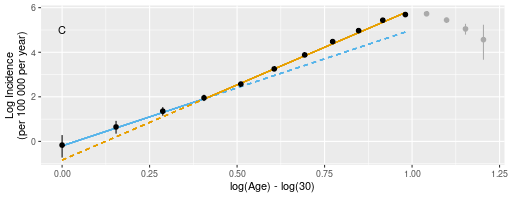
\includegraphics{multistep-model-comparison_files/figure-latex/broken-stick-figure-1.png}

\begin{Shaded}
\begin{Highlighting}[]
\KeywordTok{ggsave}\NormalTok{(}\StringTok{"plots/multistep-log-relationship-bs.pdf"}\NormalTok{,}\DataTypeTok{width=}\DecValTok{6}\NormalTok{,}\DataTypeTok{height=}\DecValTok{4}\NormalTok{)}
\KeywordTok{ggsave}\NormalTok{(}\StringTok{"plots/multistep-log-relationship-bs.png"}\NormalTok{,}\DataTypeTok{width=}\DecValTok{6}\NormalTok{,}\DataTypeTok{height=}\DecValTok{4}\NormalTok{)}
\end{Highlighting}
\end{Shaded}

\hypertarget{plot-hrc-broken-stick-model}{%
\subsection{Plot-HRC: Broken-stick
model}\label{plot-hrc-broken-stick-model}}

\begin{Shaded}
\begin{Highlighting}[]
\CommentTok{# Extract fitted values from model}
\NormalTok{values_bs =}\StringTok{ }\KeywordTok{summary}\NormalTok{(fit_bs)}\OperatorTok{$}\NormalTok{summary}

\NormalTok{m_early=values_bs[}\DecValTok{1}\NormalTok{,}\DecValTok{1}\NormalTok{]}
\NormalTok{m_late=values_bs[}\DecValTok{2}\NormalTok{,}\DecValTok{1}\NormalTok{]}
\NormalTok{bp=values_bs[}\DecValTok{3}\NormalTok{,}\DecValTok{1}\NormalTok{]}
\NormalTok{c=values_bs[}\DecValTok{4}\NormalTok{,}\DecValTok{1}\NormalTok{]}

\NormalTok{offset =}\StringTok{ }\FloatTok{0.25}

\NormalTok{x1 =}\StringTok{ }\NormalTok{start}
\NormalTok{y1 =}\StringTok{ }\NormalTok{c}\OperatorTok{+}\NormalTok{m_early}\OperatorTok{*}\NormalTok{x1}

\NormalTok{x2 =}\StringTok{ }\NormalTok{bp}
\NormalTok{y2 =}\StringTok{ }\NormalTok{c}\OperatorTok{+}\NormalTok{m_early}\OperatorTok{*}\NormalTok{x2}

\NormalTok{x2a =}\StringTok{ }\NormalTok{bp}\OperatorTok{+}\NormalTok{offset}
\NormalTok{y2a =}\StringTok{ }\NormalTok{c}\OperatorTok{+}\NormalTok{m_early}\OperatorTok{*}\NormalTok{x2a}

\NormalTok{x2b =}\StringTok{ }\NormalTok{bp}\OperatorTok{-}\NormalTok{offset}
\NormalTok{y2b =}\StringTok{ }\NormalTok{y2}\OperatorTok{-}\NormalTok{m_late}\OperatorTok{*}\NormalTok{offset}

\NormalTok{x3 =}\StringTok{ }\NormalTok{end}
\NormalTok{y3 =}\StringTok{ }\NormalTok{y2}\OperatorTok{+}\NormalTok{(end}\OperatorTok{-}\NormalTok{bp)}\OperatorTok{*}\NormalTok{m_late}

\NormalTok{x_axis <-}\StringTok{ }\KeywordTok{data.frame}\NormalTok{(}\DataTypeTok{age_label=}\KeywordTok{seq}\NormalTok{(}\DecValTok{30}\NormalTok{,}\DecValTok{100}\NormalTok{,}\DataTypeTok{by=}\DecValTok{10}\NormalTok{)) }\OperatorTok
\StringTok{  }\KeywordTok{mutate}\NormalTok{(}\DataTypeTok{age_x =} \KeywordTok{log}\NormalTok{(age_label)}\OperatorTok{-}\KeywordTok{log}\NormalTok{(}\DecValTok{30}\NormalTok{))}

\NormalTok{y_axis <-}\StringTok{ }\KeywordTok{data.frame}\NormalTok{(}\DataTypeTok{inc_label=}\KeywordTok{c}\NormalTok{(}\DecValTok{1}\NormalTok{,}\DecValTok{10}\NormalTok{,}\DecValTok{100}\NormalTok{,}\DecValTok{1000}\NormalTok{)) }\OperatorTok
\StringTok{  }\KeywordTok{mutate}\NormalTok{(}\DataTypeTok{inc_y=}\KeywordTok{log}\NormalTok{(inc_label))  }

\NormalTok{fig2_log_broken_stick_HRC <-}\StringTok{ }\NormalTok{sim_df_ms_full }\OperatorTok
\StringTok{  }\KeywordTok{ggplot}\NormalTok{(}\KeywordTok{aes}\NormalTok{(}\DataTypeTok{x=}\NormalTok{agecut5_scaled,}\DataTypeTok{y=}\NormalTok{middle_log,}
             \DataTypeTok{group=}\NormalTok{type,}\DataTypeTok{colour=}\NormalTok{restriction))}\OperatorTok{+}
\StringTok{  }\KeywordTok{geom_errorbar}\NormalTok{(}\KeywordTok{aes}\NormalTok{(}\DataTypeTok{ymin=}\NormalTok{lower_log,}\DataTypeTok{ymax=}\NormalTok{upper_log), }\DataTypeTok{width=}\DecValTok{0}\NormalTok{)}\OperatorTok{+}
\StringTok{  }\KeywordTok{scale_x_continuous}\NormalTok{(}\DataTypeTok{breaks =}\NormalTok{ x_axis}\OperatorTok{$}\NormalTok{age_x, }
                     \DataTypeTok{labels =}\NormalTok{ x_axis}\OperatorTok{$}\NormalTok{age_label,}
                     \DataTypeTok{name =} \StringTok{"Age"}\NormalTok{)}\OperatorTok{+}
\StringTok{  }\KeywordTok{scale_y_continuous}\NormalTok{(}\DataTypeTok{breaks =}\NormalTok{ y_axis}\OperatorTok{$}\NormalTok{inc_y, }
                     \DataTypeTok{labels =}\NormalTok{ y_axis}\OperatorTok{$}\NormalTok{inc_label,}
                     \DataTypeTok{limits =} \KeywordTok{c}\NormalTok{(}\OperatorTok{-}\DecValTok{1}\NormalTok{,}\DecValTok{7}\NormalTok{),}
                     \DataTypeTok{name =} \StringTok{"Incidence (per 100 000 per year)"}\NormalTok{)}\OperatorTok{+}
\StringTok{  }\KeywordTok{theme}\NormalTok{(}\DataTypeTok{legend.position =} \StringTok{"none"}\NormalTok{)}\OperatorTok{+}
\StringTok{  }\KeywordTok{geom_segment}\NormalTok{(}\DataTypeTok{x=}\NormalTok{x1,}\DataTypeTok{y=}\NormalTok{y1,}
               \DataTypeTok{xend=}\NormalTok{x2,}\DataTypeTok{yend=}\NormalTok{y2,}\DataTypeTok{colour=}\StringTok{"#56B4E9"}\NormalTok{)}\OperatorTok{+}
\StringTok{  }\KeywordTok{geom_segment}\NormalTok{(}\DataTypeTok{x=}\NormalTok{x2,}\DataTypeTok{y=}\NormalTok{y2,}
               \DataTypeTok{xend=}\NormalTok{x2a,}\DataTypeTok{yend=}\NormalTok{y2a,}\DataTypeTok{colour=}\StringTok{"#56B4E9"}\NormalTok{,}\DataTypeTok{linetype=}\StringTok{"dotted"}\NormalTok{)}\OperatorTok{+}
\StringTok{  }\KeywordTok{geom_segment}\NormalTok{(}\DataTypeTok{x=}\NormalTok{x2b,}\DataTypeTok{y=}\NormalTok{y2b,}
               \DataTypeTok{xend=}\NormalTok{x2,}\DataTypeTok{yend=}\NormalTok{y2,}\DataTypeTok{colour=}\StringTok{"#E69F00"}\NormalTok{,}\DataTypeTok{linetype=}\StringTok{"dotted"}\NormalTok{)}\OperatorTok{+}
\StringTok{  }\KeywordTok{geom_segment}\NormalTok{(}\DataTypeTok{x=}\NormalTok{x2,}\DataTypeTok{y=}\NormalTok{y2,}
               \DataTypeTok{xend=}\NormalTok{x3,}\DataTypeTok{yend=}\NormalTok{y3,}\DataTypeTok{colour=}\StringTok{"#E69F00"}\NormalTok{)}\OperatorTok{+}
\StringTok{  }\KeywordTok{geom_point}\NormalTok{(}\DataTypeTok{size=}\DecValTok{2}\NormalTok{) }\OperatorTok{+}
\StringTok{  }\KeywordTok{scale_colour_manual}\NormalTok{(}\DataTypeTok{values =}\NormalTok{ colours_modelled)}

\KeywordTok{plot}\NormalTok{(fig2_log_broken_stick_HRC)}
\end{Highlighting}
\end{Shaded}

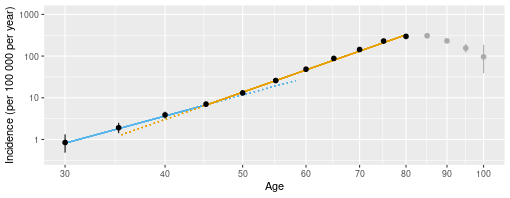
\includegraphics{multistep-model-comparison_files/figure-latex/hrc-broken-stick-figure-1.png}

\begin{Shaded}
\begin{Highlighting}[]
\KeywordTok{ggsave}\NormalTok{(}\StringTok{"plots/multistep-log-relationship-bs-HRC.pdf"}\NormalTok{,}\DataTypeTok{width=}\DecValTok{6}\NormalTok{,}\DataTypeTok{height=}\DecValTok{4}\NormalTok{)}
\KeywordTok{ggsave}\NormalTok{(}\StringTok{"plots/multistep-log-relationship-bs-HRC.png"}\NormalTok{,}\DataTypeTok{width=}\DecValTok{6}\NormalTok{,}\DataTypeTok{height=}\DecValTok{4}\NormalTok{)}
\end{Highlighting}
\end{Shaded}

\hypertarget{plot-broken-stick-model-by-sex}{%
\subsection{Plot: Broken-stick model by
sex}\label{plot-broken-stick-model-by-sex}}

\begin{Shaded}
\begin{Highlighting}[]
\CommentTok{# Extract fitted values from model}
\NormalTok{values_bs =}\StringTok{ }\KeywordTok{summary}\NormalTok{(fit_bs_sex_vc)}\OperatorTok{$}\NormalTok{summary}

\NormalTok{m_early=values_bs[}\DecValTok{1}\NormalTok{,}\DecValTok{1}\NormalTok{]}
\NormalTok{m_late=values_bs[}\DecValTok{2}\NormalTok{,}\DecValTok{1}\NormalTok{]}
\NormalTok{bp=values_bs[}\DecValTok{3}\NormalTok{,}\DecValTok{1}\NormalTok{]}
\NormalTok{c=values_bs[}\DecValTok{4}\NormalTok{,}\DecValTok{1}\NormalTok{]}
\NormalTok{c_sex=values_bs[}\DecValTok{5}\NormalTok{,}\DecValTok{1}\NormalTok{]}


\NormalTok{fig2_log_sex <-}\StringTok{ }\NormalTok{sim_df_ms_sex_full }\OperatorTok
\StringTok{  }\KeywordTok{filter}\NormalTok{(agecut5_numeric }\OperatorTok{>=}\StringTok{ }\DecValTok{30}\NormalTok{) }\OperatorTok
\StringTok{  }\KeywordTok{ggplot}\NormalTok{(}\KeywordTok{aes}\NormalTok{(}\DataTypeTok{x=}\NormalTok{agecut5_scaled,}\DataTypeTok{y=}\NormalTok{middle_log,}\DataTypeTok{group=}\NormalTok{sex,}
             \DataTypeTok{shape=}\NormalTok{sex,}\DataTypeTok{colour=}\NormalTok{sex_restriction))}\OperatorTok{+}
\StringTok{  }\KeywordTok{geom_errorbar}\NormalTok{(}\KeywordTok{aes}\NormalTok{(}\DataTypeTok{ymin=}\NormalTok{lower_log,}\DataTypeTok{ymax=}\NormalTok{upper_log), }\DataTypeTok{width=}\DecValTok{0}\NormalTok{)}\OperatorTok{+}
\StringTok{  }\KeywordTok{ylab}\NormalTok{(}\StringTok{"Log Incidence}\CharTok{\textbackslash{}n}\StringTok{(per 100 000 per year)"}\NormalTok{)}\OperatorTok{+}
\StringTok{  }\KeywordTok{xlab}\NormalTok{(}\StringTok{"log(Age) - log(30)"}\NormalTok{) }\OperatorTok{+}\StringTok{ }
\StringTok{  }\CommentTok{#theme(legend.position = c(0.8,0.2),}
\StringTok{  }\CommentTok{#                       legend.title = element_blank()) +}
\StringTok{  }\KeywordTok{theme}\NormalTok{(}\DataTypeTok{legend.position =} \StringTok{"none"}\NormalTok{) }\OperatorTok{+}\StringTok{ }
\StringTok{  }\KeywordTok{scale_color_manual}\NormalTok{(}\DataTypeTok{values =}\NormalTok{ colours_mf_modelled)}\OperatorTok{+}
\StringTok{  }\KeywordTok{geom_segment}\NormalTok{(}\DataTypeTok{x=}\NormalTok{start,}\DataTypeTok{y=}\NormalTok{c}\OperatorTok{+}\NormalTok{m_early}\OperatorTok{*}\NormalTok{start,}
               \DataTypeTok{xend=}\NormalTok{bp,}\DataTypeTok{yend=}\NormalTok{c}\OperatorTok{+}\NormalTok{m_early}\OperatorTok{*}\NormalTok{bp,}\DataTypeTok{colour=}\NormalTok{colours_mf[}\DecValTok{1}\NormalTok{])}\OperatorTok{+}
\StringTok{  }\KeywordTok{geom_segment}\NormalTok{(}\DataTypeTok{x=}\NormalTok{bp,}\DataTypeTok{y=}\NormalTok{c}\OperatorTok{+}\NormalTok{m_early}\OperatorTok{*}\NormalTok{bp,}
               \DataTypeTok{xend=}\NormalTok{end,}\DataTypeTok{yend=}\NormalTok{c}\OperatorTok{+}\NormalTok{m_early}\OperatorTok{*}\NormalTok{bp}\OperatorTok{+}\NormalTok{(end}\OperatorTok{-}\NormalTok{bp)}\OperatorTok{*}\NormalTok{m_late,}\DataTypeTok{colour=}\NormalTok{colours_mf[}\DecValTok{1}\NormalTok{])}\OperatorTok{+}
\StringTok{  }\KeywordTok{geom_segment}\NormalTok{(}\DataTypeTok{x=}\NormalTok{start,}\DataTypeTok{y=}\NormalTok{c}\OperatorTok{+}\NormalTok{c_sex}\OperatorTok{+}\NormalTok{m_early}\OperatorTok{*}\NormalTok{start,}
               \DataTypeTok{xend=}\NormalTok{bp,}\DataTypeTok{yend=}\NormalTok{c}\OperatorTok{+}\NormalTok{c_sex}\OperatorTok{+}\NormalTok{m_early}\OperatorTok{*}\NormalTok{bp,}\DataTypeTok{colour=}\NormalTok{colours_mf[}\DecValTok{2}\NormalTok{])}\OperatorTok{+}
\StringTok{  }\KeywordTok{geom_segment}\NormalTok{(}\DataTypeTok{x=}\NormalTok{bp,}\DataTypeTok{y=}\NormalTok{c}\OperatorTok{+}\NormalTok{c_sex}\OperatorTok{+}\NormalTok{m_early}\OperatorTok{*}\NormalTok{bp,}
               \DataTypeTok{xend=}\NormalTok{end,}\DataTypeTok{yend=}\NormalTok{c}\OperatorTok{+}\NormalTok{c_sex}\OperatorTok{+}\NormalTok{m_early}\OperatorTok{*}\NormalTok{bp}\OperatorTok{+}
\StringTok{                  }\NormalTok{(end}\OperatorTok{-}\NormalTok{bp)}\OperatorTok{*}\NormalTok{m_late,}\DataTypeTok{colour=}\NormalTok{colours_mf[}\DecValTok{2}\NormalTok{])}\OperatorTok{+}
\StringTok{  }\KeywordTok{guides}\NormalTok{(}\DataTypeTok{colour=}\OtherTok{FALSE}\NormalTok{) }\OperatorTok{+}
\StringTok{  }\KeywordTok{geom_point}\NormalTok{(}\DataTypeTok{size=}\DecValTok{2}\NormalTok{) }\OperatorTok{+}
\StringTok{  }\KeywordTok{annotate}\NormalTok{(}\StringTok{"text"}\NormalTok{,}\DataTypeTok{x=}\DecValTok{0}\NormalTok{,}\DataTypeTok{y=}\DecValTok{5}\NormalTok{,}\DataTypeTok{label=}\StringTok{"E"}\NormalTok{)}


\KeywordTok{print}\NormalTok{(fig2_log_sex)}
\end{Highlighting}
\end{Shaded}

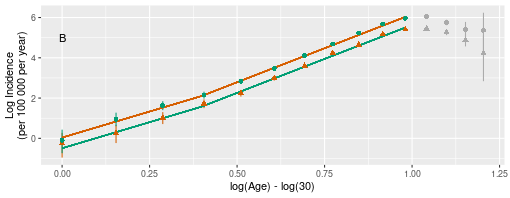
\includegraphics{multistep-model-comparison_files/figure-latex/broken-stick-sex-figure-1.png}

\begin{Shaded}
\begin{Highlighting}[]
\KeywordTok{ggsave}\NormalTok{(}\StringTok{"plots/multistep-log-relationship-sex.pdf"}\NormalTok{,}\DataTypeTok{width=}\DecValTok{6}\NormalTok{,}\DataTypeTok{height=}\DecValTok{4}\NormalTok{)}
\KeywordTok{ggsave}\NormalTok{(}\StringTok{"plots/multistep-log-relationship-sex.png"}\NormalTok{,}\DataTypeTok{width=}\DecValTok{6}\NormalTok{,}\DataTypeTok{height=}\DecValTok{4}\NormalTok{)}
\end{Highlighting}
\end{Shaded}

\hypertarget{plot-hrc-broken-stick-model-by-sex}{%
\subsection{Plot-HRC: broken-stick model by
sex}\label{plot-hrc-broken-stick-model-by-sex}}

\begin{Shaded}
\begin{Highlighting}[]
\CommentTok{# Extract fitted values from model}
\NormalTok{values_bs =}\StringTok{ }\KeywordTok{summary}\NormalTok{(fit_bs_sex_vc)}\OperatorTok{$}\NormalTok{summary}

\NormalTok{m_early=values_bs[}\DecValTok{1}\NormalTok{,}\DecValTok{1}\NormalTok{]}
\NormalTok{m_late=values_bs[}\DecValTok{2}\NormalTok{,}\DecValTok{1}\NormalTok{]}
\NormalTok{bp=values_bs[}\DecValTok{3}\NormalTok{,}\DecValTok{1}\NormalTok{]}
\NormalTok{c=values_bs[}\DecValTok{4}\NormalTok{,}\DecValTok{1}\NormalTok{]}
\NormalTok{c_sex=values_bs[}\DecValTok{5}\NormalTok{,}\DecValTok{1}\NormalTok{]}

\NormalTok{x_axis <-}\StringTok{ }\KeywordTok{data.frame}\NormalTok{(}\DataTypeTok{age_label=}\KeywordTok{seq}\NormalTok{(}\DecValTok{30}\NormalTok{,}\DecValTok{100}\NormalTok{,}\DataTypeTok{by=}\DecValTok{10}\NormalTok{)) }\OperatorTok
\StringTok{  }\KeywordTok{mutate}\NormalTok{(}\DataTypeTok{age_x =} \KeywordTok{log}\NormalTok{(age_label)}\OperatorTok{-}\KeywordTok{log}\NormalTok{(}\DecValTok{30}\NormalTok{))}

\NormalTok{y_axis <-}\StringTok{ }\KeywordTok{data.frame}\NormalTok{(}\DataTypeTok{inc_label=}\KeywordTok{c}\NormalTok{(}\DecValTok{1}\NormalTok{,}\DecValTok{10}\NormalTok{,}\DecValTok{100}\NormalTok{,}\DecValTok{1000}\NormalTok{)) }\OperatorTok
\StringTok{  }\KeywordTok{mutate}\NormalTok{(}\DataTypeTok{inc_y=}\KeywordTok{log}\NormalTok{(inc_label))  }

\NormalTok{fig2_log_sex_HRC <-}\StringTok{ }\NormalTok{sim_df_ms_sex_full }\OperatorTok
\StringTok{  }\KeywordTok{mutate}\NormalTok{(}\DataTypeTok{sex =} \KeywordTok{factor}\NormalTok{(sex,}\DataTypeTok{levels=}\KeywordTok{c}\NormalTok{(}\StringTok{"Male"}\NormalTok{,}\StringTok{"Female"}\NormalTok{))) }\OperatorTok
\StringTok{  }\KeywordTok{filter}\NormalTok{(agecut5_numeric }\OperatorTok{>=}\StringTok{ }\DecValTok{30}\NormalTok{) }\OperatorTok
\StringTok{  }\KeywordTok{ggplot}\NormalTok{(}\KeywordTok{aes}\NormalTok{(}\DataTypeTok{x=}\NormalTok{agecut5_scaled,}\DataTypeTok{y=}\NormalTok{middle_log,}\DataTypeTok{group=}\NormalTok{sex,}
             \DataTypeTok{shape=}\NormalTok{sex,}\DataTypeTok{colour=}\NormalTok{sex_restriction))}\OperatorTok{+}
\StringTok{  }\KeywordTok{geom_errorbar}\NormalTok{(}\KeywordTok{aes}\NormalTok{(}\DataTypeTok{ymin=}\NormalTok{lower_log,}\DataTypeTok{ymax=}\NormalTok{upper_log), }\DataTypeTok{width=}\DecValTok{0}\NormalTok{)}\OperatorTok{+}
\StringTok{  }\KeywordTok{scale_x_continuous}\NormalTok{(}\DataTypeTok{breaks =}\NormalTok{ x_axis}\OperatorTok{$}\NormalTok{age_x, }
                     \DataTypeTok{labels =}\NormalTok{ x_axis}\OperatorTok{$}\NormalTok{age_label,}
                     \DataTypeTok{name =} \StringTok{"Age"}\NormalTok{)}\OperatorTok{+}
\StringTok{  }\KeywordTok{scale_y_continuous}\NormalTok{(}\DataTypeTok{breaks =}\NormalTok{ y_axis}\OperatorTok{$}\NormalTok{inc_y, }
                     \DataTypeTok{labels =}\NormalTok{ y_axis}\OperatorTok{$}\NormalTok{inc_label,}
                     \DataTypeTok{limits =} \KeywordTok{c}\NormalTok{(}\OperatorTok{-}\DecValTok{1}\NormalTok{,}\DecValTok{7}\NormalTok{),}
                     \DataTypeTok{name =} \StringTok{"Incidence (per 100 000 per year)"}\NormalTok{)}\OperatorTok{+}
\StringTok{  }\KeywordTok{theme}\NormalTok{(}\DataTypeTok{legend.position =} \KeywordTok{c}\NormalTok{(}\FloatTok{0.8}\NormalTok{,}\FloatTok{0.2}\NormalTok{),}
                         \DataTypeTok{legend.title =} \KeywordTok{element_blank}\NormalTok{())}\OperatorTok{+}
\StringTok{  }\KeywordTok{guides}\NormalTok{(}\DataTypeTok{colour=}\OtherTok{FALSE}\NormalTok{) }\OperatorTok{+}
\StringTok{  }\KeywordTok{scale_color_manual}\NormalTok{(}\DataTypeTok{values =}\NormalTok{ colours_mf_modelled)}\OperatorTok{+}
\StringTok{  }\KeywordTok{geom_segment}\NormalTok{(}\DataTypeTok{x=}\NormalTok{start,}\DataTypeTok{y=}\NormalTok{c}\OperatorTok{+}\NormalTok{m_early}\OperatorTok{*}\NormalTok{start,}
               \DataTypeTok{xend=}\NormalTok{bp,}\DataTypeTok{yend=}\NormalTok{c}\OperatorTok{+}\NormalTok{m_early}\OperatorTok{*}\NormalTok{bp,}\DataTypeTok{colour=}\NormalTok{colours_mf[}\DecValTok{1}\NormalTok{])}\OperatorTok{+}
\StringTok{  }\KeywordTok{geom_segment}\NormalTok{(}\DataTypeTok{x=}\NormalTok{bp,}\DataTypeTok{y=}\NormalTok{c}\OperatorTok{+}\NormalTok{m_early}\OperatorTok{*}\NormalTok{bp,}
               \DataTypeTok{xend=}\NormalTok{end,}\DataTypeTok{yend=}\NormalTok{c}\OperatorTok{+}\NormalTok{m_early}\OperatorTok{*}\NormalTok{bp}\OperatorTok{+}\NormalTok{(end}\OperatorTok{-}\NormalTok{bp)}\OperatorTok{*}\NormalTok{m_late,}\DataTypeTok{colour=}\NormalTok{colours_mf[}\DecValTok{1}\NormalTok{])}\OperatorTok{+}
\StringTok{  }\KeywordTok{geom_segment}\NormalTok{(}\DataTypeTok{x=}\NormalTok{start,}\DataTypeTok{y=}\NormalTok{c}\OperatorTok{+}\NormalTok{c_sex}\OperatorTok{+}\NormalTok{m_early}\OperatorTok{*}\NormalTok{start,}
               \DataTypeTok{xend=}\NormalTok{bp,}\DataTypeTok{yend=}\NormalTok{c}\OperatorTok{+}\NormalTok{c_sex}\OperatorTok{+}\NormalTok{m_early}\OperatorTok{*}\NormalTok{bp,}\DataTypeTok{colour=}\NormalTok{colours_mf[}\DecValTok{2}\NormalTok{])}\OperatorTok{+}
\StringTok{  }\KeywordTok{geom_segment}\NormalTok{(}\DataTypeTok{x=}\NormalTok{bp,}\DataTypeTok{y=}\NormalTok{c}\OperatorTok{+}\NormalTok{c_sex}\OperatorTok{+}\NormalTok{m_early}\OperatorTok{*}\NormalTok{bp,}
               \DataTypeTok{xend=}\NormalTok{end,}\DataTypeTok{yend=}\NormalTok{c}\OperatorTok{+}\NormalTok{c_sex}\OperatorTok{+}\NormalTok{m_early}\OperatorTok{*}\NormalTok{bp}\OperatorTok{+}\NormalTok{(end}\OperatorTok{-}\NormalTok{bp)}\OperatorTok{*}\NormalTok{m_late,}\DataTypeTok{colour=}\NormalTok{colours_mf[}\DecValTok{2}\NormalTok{])}\OperatorTok{+}
\StringTok{  }\KeywordTok{geom_point}\NormalTok{(}\DataTypeTok{size=}\DecValTok{2}\NormalTok{)}


\KeywordTok{print}\NormalTok{(fig2_log_sex_HRC)}
\end{Highlighting}
\end{Shaded}

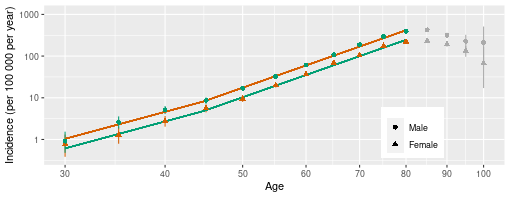
\includegraphics{multistep-model-comparison_files/figure-latex/hrc-broken-stick-sex-figure-1.png}

\begin{Shaded}
\begin{Highlighting}[]
\KeywordTok{ggsave}\NormalTok{(}\StringTok{"plots/multistep-log-relationship-sex-HRC.pdf"}\NormalTok{,}\DataTypeTok{width=}\DecValTok{6}\NormalTok{,}\DataTypeTok{height=}\DecValTok{4}\NormalTok{)}
\KeywordTok{ggsave}\NormalTok{(}\StringTok{"plots/multistep-log-relationship-sex-HRC.png"}\NormalTok{,}\DataTypeTok{width=}\DecValTok{6}\NormalTok{,}\DataTypeTok{height=}\DecValTok{4}\NormalTok{)}
\end{Highlighting}
\end{Shaded}

\hypertarget{plot-figure-2}{%
\subsection{Plot: Figure 2}\label{plot-figure-2}}

\begin{Shaded}
\begin{Highlighting}[]
\NormalTok{figure_}\DecValTok{2}\NormalTok{ =}\StringTok{ }\NormalTok{cowplot}\OperatorTok{::}\KeywordTok{plot_grid}\NormalTok{(fig2_age_specific_incidence,}
\NormalTok{                              fig2_log_linear,}
\NormalTok{                              fig2_log_broken_stick, }
\NormalTok{                              fig2_age_sex_specific_incidence,}
\NormalTok{                              fig2_log_sex, }
                              \DataTypeTok{align =} \StringTok{'v'}\NormalTok{,}
                              \DataTypeTok{axis =} \StringTok{'bt'}\NormalTok{, }\DataTypeTok{ncol =} \DecValTok{1}\NormalTok{)}

\KeywordTok{plot}\NormalTok{(figure_}\DecValTok{2}\NormalTok{)}
\end{Highlighting}
\end{Shaded}

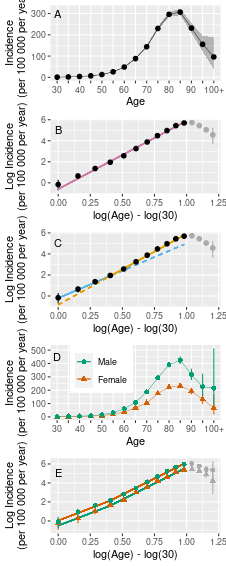
\includegraphics{multistep-model-comparison_files/figure-latex/figure2-1.png}

\begin{Shaded}
\begin{Highlighting}[]
\KeywordTok{ggsave}\NormalTok{(}\StringTok{"plots/multistep-figure-2.pdf"}\NormalTok{,}\DataTypeTok{width=}\DecValTok{4}\NormalTok{,}\DataTypeTok{height=}\DecValTok{12}\NormalTok{)}
\KeywordTok{ggsave}\NormalTok{(}\StringTok{"plots/multistep-figure-2.png"}\NormalTok{,}\DataTypeTok{width=}\DecValTok{4}\NormalTok{,}\DataTypeTok{height=}\DecValTok{12}\NormalTok{)}
\end{Highlighting}
\end{Shaded}

\hypertarget{plot-figure-3}{%
\subsection{Plot: Figure 3}\label{plot-figure-3}}

\begin{Shaded}
\begin{Highlighting}[]
\NormalTok{figure_}\DecValTok{3}\NormalTok{ =}\StringTok{ }\NormalTok{cowplot}\OperatorTok{::}\KeywordTok{plot_grid}\NormalTok{(fig2_age_sex_specific_incidence,}
\NormalTok{                              fig2_log_sex, }
                              \DataTypeTok{align =} \StringTok{'v'}\NormalTok{,}
                              \DataTypeTok{axis =} \StringTok{'bt'}\NormalTok{, }\DataTypeTok{ncol =} \DecValTok{1}\NormalTok{)}

\KeywordTok{plot}\NormalTok{(figure_}\DecValTok{3}\NormalTok{)}
\end{Highlighting}
\end{Shaded}

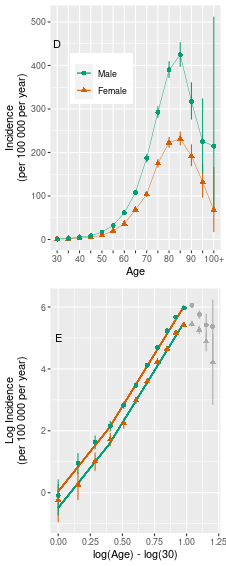
\includegraphics{multistep-model-comparison_files/figure-latex/figure3-1.png}

\begin{Shaded}
\begin{Highlighting}[]
\KeywordTok{ggsave}\NormalTok{(}\StringTok{"plots/multistep-figure-3.pdf"}\NormalTok{,}\DataTypeTok{width=}\DecValTok{4}\NormalTok{,}\DataTypeTok{height=}\DecValTok{6}\NormalTok{)}
\KeywordTok{ggsave}\NormalTok{(}\StringTok{"plots/multistep-figure-3.png"}\NormalTok{,}\DataTypeTok{width=}\DecValTok{4}\NormalTok{,}\DataTypeTok{height=}\DecValTok{6}\NormalTok{)}
\end{Highlighting}
\end{Shaded}

\hypertarget{plot-armitage-doll-model}{%
\subsection{Plot: Armitage-Doll model}\label{plot-armitage-doll-model}}

\begin{Shaded}
\begin{Highlighting}[]
\CommentTok{# Extract fitted values from model}
\NormalTok{values_ad =}\StringTok{ }\KeywordTok{summary}\NormalTok{(fit_ad)}\OperatorTok{$}\NormalTok{summary}
\NormalTok{alpha=values_ad[}\DecValTok{1}\NormalTok{,}\DecValTok{1}\NormalTok{]}
\NormalTok{k=values_ad[}\DecValTok{2}\NormalTok{,}\DecValTok{1}\NormalTok{]}

\NormalTok{simdf <-}\StringTok{ }\KeywordTok{data.frame}\NormalTok{(}\DataTypeTok{age=}\KeywordTok{seq}\NormalTok{(}\DecValTok{30}\NormalTok{,}\DecValTok{100}\NormalTok{)) }\OperatorTok
\StringTok{  }\KeywordTok{mutate}\NormalTok{(}\DataTypeTok{predinc =}\NormalTok{ (alpha}\OperatorTok{*}\NormalTok{age)}\OperatorTok{^}\NormalTok{(k}\DecValTok{-1}\NormalTok{)}\OperatorTok{*}\DecValTok{100000}\NormalTok{)}

\NormalTok{fig4_ad <-}\StringTok{ }\KeywordTok{ggplot}\NormalTok{(simdf,}\KeywordTok{aes}\NormalTok{(}\DataTypeTok{x=}\NormalTok{age,}\DataTypeTok{y=}\NormalTok{predinc))}\OperatorTok{+}\KeywordTok{geom_line}\NormalTok{(}\DataTypeTok{colour=}\StringTok{"#CC79A7"}\NormalTok{)}\OperatorTok{+}
\StringTok{  }\KeywordTok{geom_point}\NormalTok{(}\DataTypeTok{data=}\NormalTok{sim_df_ms_full,}\KeywordTok{aes}\NormalTok{(}\DataTypeTok{x=}\NormalTok{agecut5_numeric,}\DataTypeTok{y=}\NormalTok{middle))}\OperatorTok{+}
\StringTok{  }\KeywordTok{geom_errorbar}\NormalTok{(}\DataTypeTok{data=}\NormalTok{sim_df_ms_full,}\KeywordTok{aes}\NormalTok{(}\DataTypeTok{x=}\NormalTok{agecut5_numeric,}\DataTypeTok{y=}\NormalTok{middle,}\DataTypeTok{ymin=}\NormalTok{lower,}\DataTypeTok{ymax=}\NormalTok{upper), }\DataTypeTok{width=}\DecValTok{0}\NormalTok{)}\OperatorTok{+}
\StringTok{  }\KeywordTok{annotate}\NormalTok{(}\StringTok{"text"}\NormalTok{,}\DataTypeTok{x=}\DecValTok{40}\NormalTok{,}\DataTypeTok{y=}\DecValTok{1000}\NormalTok{,}\DataTypeTok{label=}\StringTok{"Armitage-Doll}\CharTok{\textbackslash{}n}\StringTok{ Model"}\NormalTok{)}\OperatorTok{+}
\StringTok{  }\KeywordTok{xlab}\NormalTok{(}\StringTok{"Age"}\NormalTok{)}\OperatorTok{+}\KeywordTok{ylab}\NormalTok{(}\StringTok{"Incidence}\CharTok{\textbackslash{}n}\StringTok{(per 100 000 per year)"}\NormalTok{)}

\KeywordTok{plot}\NormalTok{(fig4_ad)}
\end{Highlighting}
\end{Shaded}

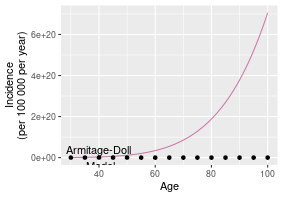
\includegraphics{multistep-model-comparison_files/figure-latex/armitage_doll-1.png}

\begin{Shaded}
\begin{Highlighting}[]
\KeywordTok{ggsave}\NormalTok{(}\StringTok{"plots/multistep-ad-fit.pdf"}\NormalTok{,}\DataTypeTok{width=}\DecValTok{5}\NormalTok{,}\DataTypeTok{height=}\DecValTok{3}\NormalTok{)}
\end{Highlighting}
\end{Shaded}

\hypertarget{plot-armitage-doll-model-by-sex}{%
\subsection{Plot: Armitage-Doll model by
Sex}\label{plot-armitage-doll-model-by-sex}}

\begin{Shaded}
\begin{Highlighting}[]
\CommentTok{# Extract fitted values from model}
\NormalTok{values_ad_sex =}\StringTok{ }\KeywordTok{summary}\NormalTok{(fit_ad_sex)}\OperatorTok{$}\NormalTok{summary}

\NormalTok{alpha=values_ad_sex[}\DecValTok{1}\NormalTok{,}\DecValTok{1}\NormalTok{]}\OperatorTok{/}\FloatTok{1e3}
\NormalTok{k=values_ad_sex[}\DecValTok{2}\NormalTok{,}\DecValTok{1}\NormalTok{]}

\NormalTok{alpha_sex=values_ad_sex[}\DecValTok{3}\NormalTok{,}\DecValTok{1}\NormalTok{]}\OperatorTok{/}\FloatTok{1e3}
\NormalTok{k_sex=values_ad_sex[}\DecValTok{4}\NormalTok{,}\DecValTok{1}\NormalTok{]}

\NormalTok{alpha1 <-}\StringTok{ }\NormalTok{alpha }\OperatorTok{+}\StringTok{ }\NormalTok{alpha_sex}
\NormalTok{k1 <-}\StringTok{ }\NormalTok{k }\OperatorTok{+}\StringTok{ }\NormalTok{k_sex}

\NormalTok{simdf <-}\StringTok{ }\KeywordTok{data.frame}\NormalTok{(}\DataTypeTok{age=}\KeywordTok{seq}\NormalTok{(}\DecValTok{30}\NormalTok{,}\DecValTok{100}\NormalTok{)) }\OperatorTok
\StringTok{  }\KeywordTok{mutate}\NormalTok{(}\DataTypeTok{predinc =}\NormalTok{ (alpha}\OperatorTok{*}\NormalTok{age)}\OperatorTok{^}\NormalTok{(k}\DecValTok{-1}\NormalTok{)}\OperatorTok{*}\DecValTok{100000}\NormalTok{)}

\NormalTok{simdf_female <-}\StringTok{ }\KeywordTok{data.frame}\NormalTok{(}\DataTypeTok{age=}\KeywordTok{seq}\NormalTok{(}\DecValTok{30}\NormalTok{,}\DecValTok{100}\NormalTok{)) }\OperatorTok
\StringTok{  }\KeywordTok{mutate}\NormalTok{(}\DataTypeTok{predinc =}\NormalTok{ (alpha1}\OperatorTok{*}\NormalTok{age)}\OperatorTok{^}\NormalTok{(k1}\DecValTok{-1}\NormalTok{)}\OperatorTok{*}\DecValTok{100000}\NormalTok{)}



\NormalTok{fig4_ad_sex <-}\StringTok{ }\NormalTok{sim_df_ms_sex_full }\OperatorTok
\StringTok{  }\KeywordTok{mutate}\NormalTok{(}\DataTypeTok{sex =} \KeywordTok{factor}\NormalTok{(sex,}\DataTypeTok{levels=}\KeywordTok{c}\NormalTok{(}\StringTok{"Male"}\NormalTok{,}\StringTok{"Female"}\NormalTok{))) }\OperatorTok
\StringTok{  }\KeywordTok{ggplot}\NormalTok{(}\KeywordTok{aes}\NormalTok{(}\DataTypeTok{x=}\NormalTok{agecut5_numeric,}\DataTypeTok{y=}\NormalTok{middle,}\DataTypeTok{colour=}\NormalTok{sex))}\OperatorTok{+}
\StringTok{  }\KeywordTok{geom_point}\NormalTok{()}\OperatorTok{+}\KeywordTok{geom_errorbar}\NormalTok{(}\KeywordTok{aes}\NormalTok{(}\DataTypeTok{ymin=}\NormalTok{lower,}\DataTypeTok{ymax=}\NormalTok{upper), }\DataTypeTok{width=}\DecValTok{0}\NormalTok{)}\OperatorTok{+}
\StringTok{  }\KeywordTok{scale_color_manual}\NormalTok{(}\DataTypeTok{values =}\NormalTok{ colours_mf)}\OperatorTok{+}
\StringTok{  }\KeywordTok{geom_line}\NormalTok{(}\DataTypeTok{data=}\NormalTok{simdf,}\KeywordTok{aes}\NormalTok{(}\DataTypeTok{x=}\NormalTok{age,}\DataTypeTok{y=}\NormalTok{predinc),}\DataTypeTok{colour=}\NormalTok{colours_mf[}\DecValTok{1}\NormalTok{])}\OperatorTok{+}
\StringTok{  }\KeywordTok{geom_line}\NormalTok{(}\DataTypeTok{data=}\NormalTok{simdf_female,}\KeywordTok{aes}\NormalTok{(}\DataTypeTok{x=}\NormalTok{age,}\DataTypeTok{y=}\NormalTok{predinc),}\DataTypeTok{colour=}\NormalTok{colours_mf[}\DecValTok{2}\NormalTok{])}\OperatorTok{+}
\StringTok{  }\KeywordTok{annotate}\NormalTok{(}\StringTok{"text"}\NormalTok{,}\DataTypeTok{x=}\DecValTok{40}\NormalTok{,}\DataTypeTok{y=}\DecValTok{600}\NormalTok{,}\DataTypeTok{label=}\StringTok{"AD Model"}\NormalTok{)}\OperatorTok{+}
\StringTok{  }\KeywordTok{xlab}\NormalTok{(}\StringTok{"Age"}\NormalTok{)}\OperatorTok{+}\KeywordTok{ylab}\NormalTok{(}\StringTok{"Incidence}\CharTok{\textbackslash{}n}\StringTok{(per 100 000 per year)"}\NormalTok{)}\OperatorTok{+}
\StringTok{  }\KeywordTok{coord_cartesian}\NormalTok{(}\DataTypeTok{ylim=}\KeywordTok{c}\NormalTok{(}\DecValTok{0}\NormalTok{, }\DecValTok{700}\NormalTok{))}\OperatorTok{+}
\StringTok{  }\KeywordTok{theme}\NormalTok{(}\DataTypeTok{legend.position =} \KeywordTok{c}\NormalTok{(}\FloatTok{0.2}\NormalTok{,}\FloatTok{0.4}\NormalTok{),}
        \DataTypeTok{legend.title =} \KeywordTok{element_blank}\NormalTok{())}

\KeywordTok{plot}\NormalTok{(fig4_ad_sex)}
\end{Highlighting}
\end{Shaded}

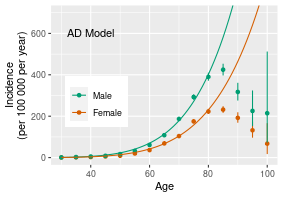
\includegraphics{multistep-model-comparison_files/figure-latex/armitage_doll_sex-1.png}

\begin{Shaded}
\begin{Highlighting}[]
\KeywordTok{ggsave}\NormalTok{(}\StringTok{"plots/multistep-ad-sex.pdf"}\NormalTok{,}\DataTypeTok{width=}\DecValTok{5}\NormalTok{,}\DataTypeTok{height=}\DecValTok{3}\NormalTok{)}
\KeywordTok{ggsave}\NormalTok{(}\StringTok{"plots/multistep-ad-sex.png"}\NormalTok{,}\DataTypeTok{width=}\DecValTok{5}\NormalTok{,}\DataTypeTok{height=}\DecValTok{3}\NormalTok{)}
\end{Highlighting}
\end{Shaded}

\hypertarget{plot-beta-model}{%
\subsection{Plot: Beta model}\label{plot-beta-model}}

\begin{Shaded}
\begin{Highlighting}[]
\CommentTok{# Fit for beta (from nls)}
\NormalTok{alpha =}\StringTok{ }\FloatTok{6.084e-03}
\NormalTok{beta =}\StringTok{ }\FloatTok{9.863e-03}
\NormalTok{k =}\StringTok{ }\FloatTok{7.202}

\CommentTok{# Extract fitted values from model}
\NormalTok{values_beta =}\StringTok{ }\KeywordTok{summary}\NormalTok{(fit_beta)}\OperatorTok{$}\NormalTok{summary}

\NormalTok{alpha=values_beta[}\DecValTok{1}\NormalTok{,}\DecValTok{1}\NormalTok{]}
\NormalTok{beta=values_beta[}\DecValTok{2}\NormalTok{,}\DecValTok{1}\NormalTok{]}
\NormalTok{k=values_beta[}\DecValTok{3}\NormalTok{,}\DecValTok{1}\NormalTok{]}

\CommentTok{#values_beta = summary(fit_beta)$c_summary}
\CommentTok{#chain = 2}

\CommentTok{#alpha=values_beta[1,1,chain]}
\CommentTok{#beta=values_beta[2,1,chain]}
\CommentTok{#k=values_beta[3,1,chain]}


\NormalTok{simdf <-}\StringTok{ }\KeywordTok{data.frame}\NormalTok{(}\DataTypeTok{age=}\KeywordTok{seq}\NormalTok{(}\DecValTok{30}\NormalTok{,}\DecValTok{100}\NormalTok{)) }\OperatorTok
\StringTok{  }\KeywordTok{mutate}\NormalTok{(}\DataTypeTok{predinc =}\NormalTok{ (alpha}\OperatorTok{*}\NormalTok{age)}\OperatorTok{^}\NormalTok{(k}\DecValTok{-1}\NormalTok{)}\OperatorTok{*}\NormalTok{(}\DecValTok{1}\OperatorTok{-}\NormalTok{beta}\OperatorTok{*}\NormalTok{age)}\OperatorTok{*}\DecValTok{100000}\NormalTok{)}

\NormalTok{fig4_beta <-}\StringTok{ }\KeywordTok{ggplot}\NormalTok{(simdf,}\KeywordTok{aes}\NormalTok{(}\DataTypeTok{x=}\NormalTok{age,}\DataTypeTok{y=}\NormalTok{predinc))}\OperatorTok{+}\KeywordTok{geom_line}\NormalTok{(}\DataTypeTok{colour=}\StringTok{"#CC79A7"}\NormalTok{)}\OperatorTok{+}
\StringTok{  }\KeywordTok{geom_point}\NormalTok{(}\DataTypeTok{data=}\NormalTok{sim_df_ms_full,}\KeywordTok{aes}\NormalTok{(}\DataTypeTok{x=}\NormalTok{agecut5_numeric,}\DataTypeTok{y=}\NormalTok{middle))}\OperatorTok{+}
\StringTok{  }\KeywordTok{geom_errorbar}\NormalTok{(}\DataTypeTok{data=}\NormalTok{sim_df_ms_full,}\KeywordTok{aes}\NormalTok{(}\DataTypeTok{x=}\NormalTok{agecut5_numeric,}\DataTypeTok{y=}\NormalTok{middle,}\DataTypeTok{ymin=}\NormalTok{lower,}\DataTypeTok{ymax=}\NormalTok{upper), }\DataTypeTok{width=}\DecValTok{0}\NormalTok{)}\OperatorTok{+}
\StringTok{  }\KeywordTok{annotate}\NormalTok{(}\StringTok{"text"}\NormalTok{,}\DataTypeTok{x=}\DecValTok{40}\NormalTok{,}\DataTypeTok{y=}\DecValTok{250}\NormalTok{,}\DataTypeTok{label=}\StringTok{"Beta}\CharTok{\textbackslash{}n}\StringTok{ Model"}\NormalTok{)}\OperatorTok{+}
\StringTok{  }\KeywordTok{xlab}\NormalTok{(}\StringTok{"Age"}\NormalTok{)}\OperatorTok{+}\KeywordTok{ylab}\NormalTok{(}\StringTok{"Incidence}\CharTok{\textbackslash{}n}\StringTok{(per 100 000 per year)"}\NormalTok{)}

\KeywordTok{plot}\NormalTok{(fig4_beta)}
\end{Highlighting}
\end{Shaded}

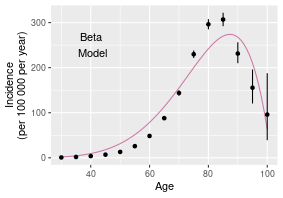
\includegraphics{multistep-model-comparison_files/figure-latex/beta-1.png}

\begin{Shaded}
\begin{Highlighting}[]
\KeywordTok{ggsave}\NormalTok{(}\StringTok{"plots/multistep-beta-fit.pdf"}\NormalTok{,}\DataTypeTok{width=}\DecValTok{5}\NormalTok{,}\DataTypeTok{height=}\DecValTok{3}\NormalTok{)}
\end{Highlighting}
\end{Shaded}

\hypertarget{plot-beta-model-by-sex}{%
\subsection{Plot: Beta model by Sex}\label{plot-beta-model-by-sex}}

\begin{Shaded}
\begin{Highlighting}[]
\CommentTok{# Extract fitted values from model}
\NormalTok{values_beta_sex =}\StringTok{ }\KeywordTok{summary}\NormalTok{(fit_beta_sex)}\OperatorTok{$}\NormalTok{summary}

\NormalTok{alpha=values_beta_sex[}\DecValTok{1}\NormalTok{,}\DecValTok{1}\NormalTok{]}\OperatorTok{/}\FloatTok{1e3}
\NormalTok{beta=values_beta_sex[}\DecValTok{2}\NormalTok{,}\DecValTok{1}\NormalTok{]}
\NormalTok{k=values_beta_sex[}\DecValTok{3}\NormalTok{,}\DecValTok{1}\NormalTok{]}

\NormalTok{alpha_sex=values_beta_sex[}\DecValTok{4}\NormalTok{,}\DecValTok{1}\NormalTok{]}\OperatorTok{/}\FloatTok{1e3}
\NormalTok{beta_sex=values_beta_sex[}\DecValTok{5}\NormalTok{,}\DecValTok{1}\NormalTok{]}
\NormalTok{k_sex=values_beta_sex[}\DecValTok{6}\NormalTok{,}\DecValTok{1}\NormalTok{]}

\NormalTok{alpha1 <-}\StringTok{ }\NormalTok{alpha }\OperatorTok{+}\StringTok{ }\NormalTok{alpha_sex}
\NormalTok{k1 <-}\StringTok{ }\NormalTok{k }\OperatorTok{+}\StringTok{ }\NormalTok{k_sex}
\NormalTok{beta1 <-}\StringTok{ }\NormalTok{beta }\OperatorTok{+}\StringTok{ }\NormalTok{beta_sex}

\NormalTok{simdf <-}\StringTok{ }\KeywordTok{data.frame}\NormalTok{(}\DataTypeTok{age=}\KeywordTok{seq}\NormalTok{(}\DecValTok{30}\NormalTok{,}\DecValTok{100}\NormalTok{)) }\OperatorTok
\StringTok{  }\KeywordTok{mutate}\NormalTok{(}\DataTypeTok{predinc =}\NormalTok{ (alpha}\OperatorTok{*}\NormalTok{age)}\OperatorTok{^}\NormalTok{(k}\DecValTok{-1}\NormalTok{)}\OperatorTok{*}\NormalTok{(}\DecValTok{1}\OperatorTok{-}\NormalTok{beta}\OperatorTok{*}\NormalTok{age)}\OperatorTok{*}\DecValTok{100000}\NormalTok{)}

\NormalTok{simdf_female <-}\StringTok{ }\KeywordTok{data.frame}\NormalTok{(}\DataTypeTok{age=}\KeywordTok{seq}\NormalTok{(}\DecValTok{30}\NormalTok{,}\DecValTok{100}\NormalTok{)) }\OperatorTok
\StringTok{  }\KeywordTok{mutate}\NormalTok{(}\DataTypeTok{predinc =}\NormalTok{ (alpha1}\OperatorTok{*}\NormalTok{age)}\OperatorTok{^}\NormalTok{(k1}\DecValTok{-1}\NormalTok{)}\OperatorTok{*}\NormalTok{(}\DecValTok{1}\OperatorTok{-}\NormalTok{beta1}\OperatorTok{*}\NormalTok{age)}\OperatorTok{*}\DecValTok{100000}\NormalTok{)}

\NormalTok{fig4_beta_sex <-}\StringTok{ }\NormalTok{sim_df_ms_sex_full }\OperatorTok
\StringTok{  }\KeywordTok{mutate}\NormalTok{(}\DataTypeTok{sex =} \KeywordTok{factor}\NormalTok{(sex,}\DataTypeTok{levels=}\KeywordTok{c}\NormalTok{(}\StringTok{"Male"}\NormalTok{,}\StringTok{"Female"}\NormalTok{))) }\OperatorTok
\StringTok{  }\KeywordTok{ggplot}\NormalTok{(}\KeywordTok{aes}\NormalTok{(}\DataTypeTok{x=}\NormalTok{agecut5_numeric,}\DataTypeTok{y=}\NormalTok{middle,}\DataTypeTok{colour=}\NormalTok{sex))}\OperatorTok{+}
\StringTok{  }\KeywordTok{geom_point}\NormalTok{()}\OperatorTok{+}\KeywordTok{geom_errorbar}\NormalTok{(}\KeywordTok{aes}\NormalTok{(}\DataTypeTok{ymin=}\NormalTok{lower,}\DataTypeTok{ymax=}\NormalTok{upper), }\DataTypeTok{width=}\DecValTok{0}\NormalTok{)}\OperatorTok{+}
\StringTok{  }\KeywordTok{scale_color_manual}\NormalTok{(}\DataTypeTok{values =}\NormalTok{ colours_mf)}\OperatorTok{+}
\StringTok{  }\KeywordTok{geom_line}\NormalTok{(}\DataTypeTok{data=}\NormalTok{simdf,}\KeywordTok{aes}\NormalTok{(}\DataTypeTok{x=}\NormalTok{age,}\DataTypeTok{y=}\NormalTok{predinc),}\DataTypeTok{colour=}\NormalTok{colours_mf[}\DecValTok{1}\NormalTok{])}\OperatorTok{+}
\StringTok{  }\KeywordTok{geom_line}\NormalTok{(}\DataTypeTok{data=}\NormalTok{simdf_female,}\KeywordTok{aes}\NormalTok{(}\DataTypeTok{x=}\NormalTok{age,}\DataTypeTok{y=}\NormalTok{predinc),}\DataTypeTok{colour=}\NormalTok{colours_mf[}\DecValTok{2}\NormalTok{])}\OperatorTok{+}
\StringTok{  }\KeywordTok{annotate}\NormalTok{(}\StringTok{"text"}\NormalTok{,}\DataTypeTok{x=}\DecValTok{40}\NormalTok{,}\DataTypeTok{y=}\DecValTok{600}\NormalTok{,}\DataTypeTok{label=}\StringTok{"Beta Model"}\NormalTok{)}\OperatorTok{+}
\StringTok{  }\KeywordTok{xlab}\NormalTok{(}\StringTok{"Age"}\NormalTok{)}\OperatorTok{+}\KeywordTok{ylab}\NormalTok{(}\StringTok{"Incidence}\CharTok{\textbackslash{}n}\StringTok{(per 100 000 per year)"}\NormalTok{)}\OperatorTok{+}
\StringTok{  }\KeywordTok{coord_cartesian}\NormalTok{(}\DataTypeTok{ylim=}\KeywordTok{c}\NormalTok{(}\DecValTok{0}\NormalTok{, }\DecValTok{700}\NormalTok{))}\OperatorTok{+}
\StringTok{  }\KeywordTok{theme}\NormalTok{(}\DataTypeTok{legend.position =} \StringTok{"none"}\NormalTok{)}

\KeywordTok{plot}\NormalTok{(fig4_beta_sex)}
\end{Highlighting}
\end{Shaded}

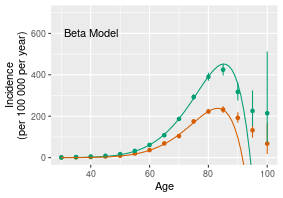
\includegraphics{multistep-model-comparison_files/figure-latex/beta_sex-1.png}

\begin{Shaded}
\begin{Highlighting}[]
\KeywordTok{ggsave}\NormalTok{(}\StringTok{"plots/multistep-beta-sex.pdf"}\NormalTok{,}\DataTypeTok{width=}\DecValTok{5}\NormalTok{,}\DataTypeTok{height=}\DecValTok{3}\NormalTok{)}
\KeywordTok{ggsave}\NormalTok{(}\StringTok{"plots/multistep-beta-sex.png"}\NormalTok{,}\DataTypeTok{width=}\DecValTok{5}\NormalTok{,}\DataTypeTok{height=}\DecValTok{3}\NormalTok{)}
\end{Highlighting}
\end{Shaded}

\hypertarget{plot-susceptibility}{%
\subsection{Plot: Susceptibility}\label{plot-susceptibility}}

\begin{Shaded}
\begin{Highlighting}[]
\CommentTok{# nls}
\CommentTok{#alpha = 1.2e-15}
\CommentTok{#C = 8.024e-02}
\CommentTok{#k = 8.2}

\CommentTok{# stan}
\NormalTok{alpha =}\StringTok{ }\FloatTok{2.03e-15}
\NormalTok{C =}\StringTok{ }\FloatTok{8.06e-02}
\NormalTok{k =}\StringTok{ }\FloatTok{8.11}

\CommentTok{# Extract fitted values from model}
\NormalTok{values_suscept =}\StringTok{ }\KeywordTok{summary}\NormalTok{(fit_suscept)}\OperatorTok{$}\NormalTok{summary}

\NormalTok{alpha=values_suscept[}\DecValTok{1}\NormalTok{,}\DecValTok{1}\NormalTok{]}\OperatorTok{/}\FloatTok{1e15}
\NormalTok{C=values_suscept[}\DecValTok{2}\NormalTok{,}\DecValTok{1}\NormalTok{]}\OperatorTok{/}\DecValTok{100}
\NormalTok{k=values_suscept[}\DecValTok{3}\NormalTok{,}\DecValTok{1}\NormalTok{]}

\NormalTok{simdf <-}\StringTok{ }\KeywordTok{data.frame}\NormalTok{(}\DataTypeTok{age=}\KeywordTok{seq}\NormalTok{(}\DecValTok{30}\NormalTok{,}\DecValTok{100}\NormalTok{)) }\OperatorTok
\StringTok{  }\KeywordTok{mutate}\NormalTok{(}\DataTypeTok{predinc =}\NormalTok{ alpha}\OperatorTok{*}\NormalTok{age}\OperatorTok{^}\NormalTok{(k}\DecValTok{-1}\NormalTok{)}\OperatorTok{*}\DecValTok{100000}\OperatorTok{/}\NormalTok{(}\DecValTok{1}\OperatorTok{+}\NormalTok{((}\DecValTok{1}\OperatorTok{-}\NormalTok{C)}\OperatorTok{/}\NormalTok{C)}\OperatorTok{*}\KeywordTok{exp}\NormalTok{(alpha}\OperatorTok{/}\NormalTok{k}\OperatorTok{*}\NormalTok{(age}\OperatorTok{^}\NormalTok{k}\DecValTok{-1}\NormalTok{))))}

\NormalTok{fig4_susceptibility <-}\StringTok{ }\KeywordTok{ggplot}\NormalTok{(simdf,}\KeywordTok{aes}\NormalTok{(}\DataTypeTok{x=}\NormalTok{age,}\DataTypeTok{y=}\NormalTok{predinc))}\OperatorTok{+}\KeywordTok{geom_line}\NormalTok{(}\DataTypeTok{colour=}\StringTok{"#CC79A7"}\NormalTok{)}\OperatorTok{+}
\StringTok{  }\KeywordTok{geom_point}\NormalTok{(}\DataTypeTok{data=}\NormalTok{sim_df_ms_full,}\KeywordTok{aes}\NormalTok{(}\DataTypeTok{x=}\NormalTok{agecut5_numeric,}\DataTypeTok{y=}\NormalTok{middle))}\OperatorTok{+}
\StringTok{  }\KeywordTok{geom_errorbar}\NormalTok{(}\DataTypeTok{data=}\NormalTok{sim_df_ms_full,}\KeywordTok{aes}\NormalTok{(}\DataTypeTok{x=}\NormalTok{agecut5_numeric,}\DataTypeTok{y=}\NormalTok{middle,}\DataTypeTok{ymin=}\NormalTok{lower,}\DataTypeTok{ymax=}\NormalTok{upper), }\DataTypeTok{width=}\DecValTok{0}\NormalTok{)}\OperatorTok{+}
\StringTok{  }\KeywordTok{annotate}\NormalTok{(}\StringTok{"text"}\NormalTok{,}\DataTypeTok{x=}\DecValTok{40}\NormalTok{,}\DataTypeTok{y=}\DecValTok{250}\NormalTok{,}\DataTypeTok{label=}\StringTok{"Susceptibility}\CharTok{\textbackslash{}n}\StringTok{ Model"}\NormalTok{)}\OperatorTok{+}
\StringTok{  }\KeywordTok{xlab}\NormalTok{(}\StringTok{"Age"}\NormalTok{)}\OperatorTok{+}\KeywordTok{ylab}\NormalTok{(}\StringTok{"Incidence}\CharTok{\textbackslash{}n}\StringTok{(per 100 000 per year)"}\NormalTok{)}

\KeywordTok{plot}\NormalTok{(fig4_susceptibility)}
\end{Highlighting}
\end{Shaded}

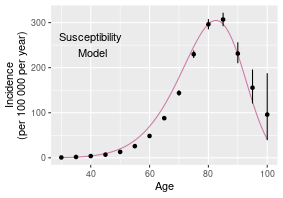
\includegraphics{multistep-model-comparison_files/figure-latex/susceptibility-1.png}

\begin{Shaded}
\begin{Highlighting}[]
\KeywordTok{ggsave}\NormalTok{(}\StringTok{"plots/multistep-susceptibiliy.pdf"}\NormalTok{,}\DataTypeTok{width=}\DecValTok{5}\NormalTok{,}\DataTypeTok{height=}\DecValTok{3}\NormalTok{)}
\end{Highlighting}
\end{Shaded}

\hypertarget{plot-susceptibility-fixed}{%
\subsection{Plot: Susceptibility
Fixed}\label{plot-susceptibility-fixed}}

\begin{Shaded}
\begin{Highlighting}[]
\CommentTok{# Extract fitted values from model}
\NormalTok{values_suscept =}\StringTok{ }\KeywordTok{summary}\NormalTok{(fit_suscept_fixed)}\OperatorTok{$}\NormalTok{summary}

\NormalTok{alpha=values_suscept[}\DecValTok{1}\NormalTok{,}\DecValTok{1}\NormalTok{]}\OperatorTok{/}\FloatTok{1e15}
\NormalTok{k=values_suscept[}\DecValTok{2}\NormalTok{,}\DecValTok{1}\NormalTok{]}
\NormalTok{C=data_list_suscept_fixed}\OperatorTok{$}\NormalTok{C}\OperatorTok{/}\DecValTok{100}


\NormalTok{simdf <-}\StringTok{ }\KeywordTok{data.frame}\NormalTok{(}\DataTypeTok{age=}\KeywordTok{seq}\NormalTok{(}\DecValTok{30}\NormalTok{,}\DecValTok{100}\NormalTok{)) }\OperatorTok
\StringTok{  }\KeywordTok{mutate}\NormalTok{(}\DataTypeTok{predinc =}\NormalTok{ alpha}\OperatorTok{*}\NormalTok{age}\OperatorTok{^}\NormalTok{(k}\DecValTok{-1}\NormalTok{)}\OperatorTok{*}\DecValTok{100000}\OperatorTok{/}\NormalTok{(}\DecValTok{1}\OperatorTok{+}\NormalTok{((}\DecValTok{1}\OperatorTok{-}\NormalTok{C)}\OperatorTok{/}\NormalTok{C)}\OperatorTok{*}\KeywordTok{exp}\NormalTok{(alpha}\OperatorTok{/}\NormalTok{k}\OperatorTok{*}\NormalTok{(age}\OperatorTok{^}\NormalTok{k}\DecValTok{-1}\NormalTok{))))}

\NormalTok{fig4_susceptibility_fixed <-}\StringTok{ }\KeywordTok{ggplot}\NormalTok{(simdf,}\KeywordTok{aes}\NormalTok{(}\DataTypeTok{x=}\NormalTok{age,}\DataTypeTok{y=}\NormalTok{predinc))}\OperatorTok{+}\KeywordTok{geom_line}\NormalTok{(}\DataTypeTok{colour=}\StringTok{"#CC79A7"}\NormalTok{)}\OperatorTok{+}
\StringTok{  }\KeywordTok{geom_point}\NormalTok{(}\DataTypeTok{data=}\NormalTok{sim_df_ms_full,}\KeywordTok{aes}\NormalTok{(}\DataTypeTok{x=}\NormalTok{agecut5_numeric,}\DataTypeTok{y=}\NormalTok{middle))}\OperatorTok{+}
\StringTok{  }\KeywordTok{geom_errorbar}\NormalTok{(}\DataTypeTok{data=}\NormalTok{sim_df_ms_full,}\KeywordTok{aes}\NormalTok{(}\DataTypeTok{x=}\NormalTok{agecut5_numeric,}\DataTypeTok{y=}\NormalTok{middle,}\DataTypeTok{ymin=}\NormalTok{lower,}\DataTypeTok{ymax=}\NormalTok{upper), }\DataTypeTok{width=}\DecValTok{0}\NormalTok{)}\OperatorTok{+}
\StringTok{  }\KeywordTok{annotate}\NormalTok{(}\StringTok{"text"}\NormalTok{,}\DataTypeTok{x=}\DecValTok{40}\NormalTok{,}\DataTypeTok{y=}\DecValTok{250}\NormalTok{,}\DataTypeTok{label=}\StringTok{"Susceptibility}\CharTok{\textbackslash{}n}\StringTok{ Model"}\NormalTok{)}\OperatorTok{+}
\StringTok{  }\KeywordTok{xlab}\NormalTok{(}\StringTok{"Age"}\NormalTok{)}\OperatorTok{+}\KeywordTok{ylab}\NormalTok{(}\StringTok{"Incidence}\CharTok{\textbackslash{}n}\StringTok{(per 100 000 per year)"}\NormalTok{)}

\KeywordTok{plot}\NormalTok{(fig4_susceptibility_fixed)}
\end{Highlighting}
\end{Shaded}

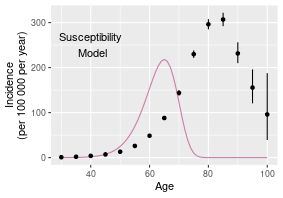
\includegraphics{multistep-model-comparison_files/figure-latex/susceptibility_fixed_C-1.png}

\begin{Shaded}
\begin{Highlighting}[]
\KeywordTok{ggsave}\NormalTok{(}\StringTok{"plots/multistep-susceptibiliy-fixed-C-03.pdf"}\NormalTok{,}\DataTypeTok{width=}\DecValTok{5}\NormalTok{,}\DataTypeTok{height=}\DecValTok{3}\NormalTok{)}
\end{Highlighting}
\end{Shaded}

\hypertarget{plot-susceptibility-model-by-sex}{%
\subsection{Plot: Susceptibility model by
Sex}\label{plot-susceptibility-model-by-sex}}

\begin{Shaded}
\begin{Highlighting}[]
\CommentTok{# nls}
\CommentTok{#alpha = 1.2e-15}
\CommentTok{#C = 8.024e-02}
\CommentTok{#k = 8.2}

\CommentTok{# stan}
\NormalTok{alpha =}\StringTok{ }\FloatTok{2.03e-15}
\NormalTok{C =}\StringTok{ }\FloatTok{8.06e-02}
\NormalTok{k =}\StringTok{ }\FloatTok{8.11}

\CommentTok{# Extract fitted values from model}
\NormalTok{values_suscept_sex =}\StringTok{ }\KeywordTok{summary}\NormalTok{(fit_suscept_sex)}\OperatorTok{$}\NormalTok{summary}

\NormalTok{alpha=values_suscept_sex[}\DecValTok{1}\NormalTok{,}\DecValTok{1}\NormalTok{]}\OperatorTok{/}\FloatTok{1e15}
\NormalTok{C=values_suscept_sex[}\DecValTok{2}\NormalTok{,}\DecValTok{1}\NormalTok{]}\OperatorTok{/}\DecValTok{100}
\NormalTok{k=values_suscept_sex[}\DecValTok{3}\NormalTok{,}\DecValTok{1}\NormalTok{]}

\NormalTok{alpha_sex=values_suscept_sex[}\DecValTok{4}\NormalTok{,}\DecValTok{1}\NormalTok{]}\OperatorTok{/}\FloatTok{1e15}
\NormalTok{C_sex=values_suscept_sex[}\DecValTok{5}\NormalTok{,}\DecValTok{1}\NormalTok{]}\OperatorTok{/}\DecValTok{100}
\NormalTok{k_sex=values_suscept_sex[}\DecValTok{6}\NormalTok{,}\DecValTok{1}\NormalTok{]}

\NormalTok{alpha1 <-}\StringTok{ }\NormalTok{(alpha }\OperatorTok{+}\StringTok{ }\NormalTok{alpha_sex)}\OperatorTok{*}\FloatTok{0.8}
\NormalTok{C1 <-}\StringTok{ }\NormalTok{C }\OperatorTok{+}\StringTok{ }\NormalTok{C_sex}
\NormalTok{k1 <-}\StringTok{ }\NormalTok{k }\OperatorTok{+}\StringTok{ }\NormalTok{k_sex}

\NormalTok{simdf <-}\StringTok{ }\KeywordTok{data.frame}\NormalTok{(}\DataTypeTok{age=}\KeywordTok{seq}\NormalTok{(}\DecValTok{30}\NormalTok{,}\DecValTok{100}\NormalTok{)) }\OperatorTok
\StringTok{  }\KeywordTok{mutate}\NormalTok{(}\DataTypeTok{predinc =}\NormalTok{ alpha}\OperatorTok{*}\NormalTok{age}\OperatorTok{^}\NormalTok{(k}\DecValTok{-1}\NormalTok{)}\OperatorTok{*}\DecValTok{100000}\OperatorTok{/}\NormalTok{(}\DecValTok{1}\OperatorTok{+}\NormalTok{((}\DecValTok{1}\OperatorTok{-}\NormalTok{C)}\OperatorTok{/}\NormalTok{C)}\OperatorTok{*}\KeywordTok{exp}\NormalTok{(alpha}\OperatorTok{/}\NormalTok{k}\OperatorTok{*}\NormalTok{(age}\OperatorTok{^}\NormalTok{k}\DecValTok{-1}\NormalTok{))))}

\NormalTok{simdf_female <-}\StringTok{ }\KeywordTok{data.frame}\NormalTok{(}\DataTypeTok{age=}\KeywordTok{seq}\NormalTok{(}\DecValTok{30}\NormalTok{,}\DecValTok{100}\NormalTok{)) }\OperatorTok
\StringTok{  }\KeywordTok{mutate}\NormalTok{(}\DataTypeTok{predinc =}\NormalTok{ alpha1}\OperatorTok{*}\NormalTok{age}\OperatorTok{^}\NormalTok{(k1}\DecValTok{-1}\NormalTok{)}\OperatorTok{*}\DecValTok{100000}\OperatorTok{/}\NormalTok{(}\DecValTok{1}\OperatorTok{+}\NormalTok{((}\DecValTok{1}\OperatorTok{-}\NormalTok{C1)}\OperatorTok{/}\NormalTok{C1)}\OperatorTok{*}\KeywordTok{exp}\NormalTok{(alpha1}\OperatorTok{/}\NormalTok{k1}\OperatorTok{*}\NormalTok{(age}\OperatorTok{^}\NormalTok{k1}\DecValTok{-1}\NormalTok{))))}



\NormalTok{fig4_susceptibility_sex <-}\StringTok{ }\NormalTok{sim_df_ms_sex_full }\OperatorTok
\StringTok{  }\KeywordTok{mutate}\NormalTok{(}\DataTypeTok{sex =} \KeywordTok{factor}\NormalTok{(sex,}\DataTypeTok{levels=}\KeywordTok{c}\NormalTok{(}\StringTok{"Male"}\NormalTok{,}\StringTok{"Female"}\NormalTok{))) }\OperatorTok
\StringTok{  }\KeywordTok{ggplot}\NormalTok{(}\KeywordTok{aes}\NormalTok{(}\DataTypeTok{x=}\NormalTok{agecut5_numeric,}\DataTypeTok{y=}\NormalTok{middle,}\DataTypeTok{colour=}\NormalTok{sex))}\OperatorTok{+}
\StringTok{  }\KeywordTok{geom_point}\NormalTok{()}\OperatorTok{+}\KeywordTok{geom_errorbar}\NormalTok{(}\KeywordTok{aes}\NormalTok{(}\DataTypeTok{ymin=}\NormalTok{lower,}\DataTypeTok{ymax=}\NormalTok{upper), }\DataTypeTok{width=}\DecValTok{0}\NormalTok{)}\OperatorTok{+}
\StringTok{  }\KeywordTok{scale_color_manual}\NormalTok{(}\DataTypeTok{values =}\NormalTok{ colours_mf)}\OperatorTok{+}
\StringTok{  }\KeywordTok{geom_line}\NormalTok{(}\DataTypeTok{data=}\NormalTok{simdf,}\KeywordTok{aes}\NormalTok{(}\DataTypeTok{x=}\NormalTok{age,}\DataTypeTok{y=}\NormalTok{predinc),}\DataTypeTok{colour=}\NormalTok{colours_mf[}\DecValTok{1}\NormalTok{])}\OperatorTok{+}
\StringTok{  }\KeywordTok{geom_line}\NormalTok{(}\DataTypeTok{data=}\NormalTok{simdf_female,}\KeywordTok{aes}\NormalTok{(}\DataTypeTok{x=}\NormalTok{age,}\DataTypeTok{y=}\NormalTok{predinc),}\DataTypeTok{colour=}\NormalTok{colours_mf[}\DecValTok{2}\NormalTok{])}\OperatorTok{+}
\StringTok{  }\KeywordTok{annotate}\NormalTok{(}\StringTok{"text"}\NormalTok{,}\DataTypeTok{x=}\DecValTok{40}\NormalTok{,}\DataTypeTok{y=}\DecValTok{600}\NormalTok{,}\DataTypeTok{label=}\StringTok{"Susceptibility}\CharTok{\textbackslash{}n}\StringTok{ Model"}\NormalTok{)}\OperatorTok{+}
\StringTok{  }\KeywordTok{xlab}\NormalTok{(}\StringTok{"Age"}\NormalTok{)}\OperatorTok{+}\KeywordTok{ylab}\NormalTok{(}\StringTok{"Incidence}\CharTok{\textbackslash{}n}\StringTok{(per 100 000 per year)"}\NormalTok{)}\OperatorTok{+}
\StringTok{  }\KeywordTok{coord_cartesian}\NormalTok{(}\DataTypeTok{ylim=}\KeywordTok{c}\NormalTok{(}\DecValTok{0}\NormalTok{, }\DecValTok{700}\NormalTok{))}\OperatorTok{+}
\StringTok{  }\KeywordTok{theme}\NormalTok{(}\DataTypeTok{legend.position =} \StringTok{"none"}\NormalTok{)}

\KeywordTok{plot}\NormalTok{(fig4_susceptibility_sex)}
\end{Highlighting}
\end{Shaded}

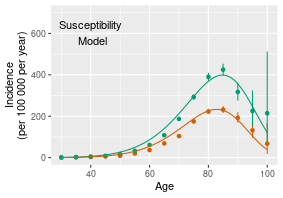
\includegraphics{multistep-model-comparison_files/figure-latex/susceptibility_sex-1.png}

\begin{Shaded}
\begin{Highlighting}[]
\KeywordTok{ggsave}\NormalTok{(}\StringTok{"plots/multistep-susceptibiliy-sex.pdf"}\NormalTok{,}\DataTypeTok{width=}\DecValTok{5}\NormalTok{,}\DataTypeTok{height=}\DecValTok{3}\NormalTok{)}
\KeywordTok{ggsave}\NormalTok{(}\StringTok{"plots/multistep-susceptibiliy-sex.png"}\NormalTok{,}\DataTypeTok{width=}\DecValTok{5}\NormalTok{,}\DataTypeTok{height=}\DecValTok{3}\NormalTok{)}
\end{Highlighting}
\end{Shaded}

\hypertarget{plot-figure-4}{%
\subsection{Plot: Figure 4}\label{plot-figure-4}}

\begin{Shaded}
\begin{Highlighting}[]
\NormalTok{figure_}\DecValTok{4}\NormalTok{ =}\StringTok{ }\NormalTok{cowplot}\OperatorTok{::}\KeywordTok{plot_grid}\NormalTok{(fig4_ad_sex,}
\NormalTok{                              fig4_beta_sex,}
\NormalTok{                              fig4_susceptibility_sex,}
                              \DataTypeTok{align =} \StringTok{'v'}\NormalTok{,}
                              \DataTypeTok{axis =} \StringTok{'bt'}\NormalTok{, }\DataTypeTok{ncol =} \DecValTok{1}\NormalTok{)}

\KeywordTok{plot}\NormalTok{(figure_}\DecValTok{4}\NormalTok{)}
\end{Highlighting}
\end{Shaded}

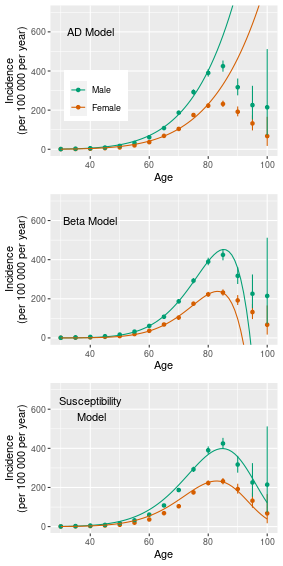
\includegraphics{multistep-model-comparison_files/figure-latex/figure4-1.png}

\begin{Shaded}
\begin{Highlighting}[]
\KeywordTok{ggsave}\NormalTok{(}\StringTok{"plots/multistep-figure-4.pdf"}\NormalTok{,}\DataTypeTok{width=}\DecValTok{4}\NormalTok{,}\DataTypeTok{height=}\DecValTok{8}\NormalTok{)}
\KeywordTok{ggsave}\NormalTok{(}\StringTok{"plots/multistep-figure-4.png"}\NormalTok{,}\DataTypeTok{width=}\DecValTok{4}\NormalTok{,}\DataTypeTok{height=}\DecValTok{8}\NormalTok{)}
\end{Highlighting}
\end{Shaded}

\end{document}
